\documentclass[12pt,letterpaper]{article}
\usepackage[top=0.85in,left=1in,footskip=0.75in,marginparwidth=2in]{geometry}

% use Unicode characters - try changing the option if you run into troubles with special characters (e.g. umlauts)
\usepackage[utf8]{inputenc}

% clean citations
\usepackage{cite}

% hyperref makes references clicky. use \url{www.example.com} or \href{www.example.com}{description} to add a clicky url
\usepackage{nameref,hyperref}

% line numbers
\usepackage[right]{lineno}
\linenumbers

% improves typesetting in LaTeX
\usepackage{microtype}
\DisableLigatures[f]{encoding = *, family = * }

% text layout - change as needed
\raggedright
\setlength{\parindent}{0.5cm}
\textwidth 6.5in 
\textheight 9in
\renewcommand{\baselinestretch}{1.5}

% use adjustwidth environment to exceed text width (see examples in text)
\usepackage{changepage}

% adjust caption style
\usepackage[font=small,aboveskip=1pt,labelfont=bf,labelsep=period,singlelinecheck=off]{caption}

% remove brackets from references
\makeatletter
\renewcommand{\@biblabel}[1]{\quad#1.}
\makeatother

% headrule, footrule and page numbers
\usepackage{lastpage,fancyhdr,graphicx}
\usepackage{epstopdf}
\pagestyle{myheadings}
\pagestyle{fancy}
\fancyhf{}
\rfoot{\thepage/\pageref{LastPage}}
\renewcommand{\footrule}{\hrule height 2pt \vspace{2mm}}
\fancyheadoffset[L]{2.25in}
\fancyfootoffset[L]{2.25in}

% use \textcolor{color}{text} for colored text (e.g. highlight to-do areas)
\usepackage{color}

% define custom colors (this one is for figure captions)
\definecolor{Gray}{gray}{.25}

% this is required to include graphics
\usepackage{graphicx}
\usepackage{subcaption}
\usepackage{pdflscape}
\graphicspath{{../figures/panels/}}

% use if you want to put caption to the side of the figure - see example in text
\usepackage{sidecap}

% use for have text wrap around figures
\usepackage{wrapfig}
\usepackage[pscoord]{eso-pic}
\usepackage[fulladjust]{marginnote}
\reversemarginpar
\usepackage{amsmath}
\usepackage{pdfpages}

% document begins here
\begin{document}
\vspace*{0.35in}

% title goes here:
\begin{flushleft}
{\Large
\textbf{Investigating essential genes in Enterobacteriaceae using
transposon insertion sequencing}
}
\newline
% authors go here:
\\
%Fatemeh Ashari Ghomi\textsuperscript{1},
%Paul P. Gardner\textsuperscript{1,*},
%Lars Barquist\textsuperscript{2}
%\\
%\bigskip
%\bf{1} University of Canterbury
%\\
%\bf{2} Wurzburg University
%\\
%\bigskip
%* paul.gardner@canterbury.ac.nz

\end{flushleft}% Correct contributions, italicise bacteria names, italicise gene names, abbreviate species names
% convert MG1655(keio) to BW25113    http://mbio.asm.org/content/6/3/e00306-15.full#sec-11
% EC958 -> CFT073    http://journals.plos.org/plospathogens/article?id=10.1371/journal.ppat.1003788#ppat.1003788.s003
\section{Abstract}
The study of genes that are essential for the survival of a prokaryotic organism can help with the design of new antibiotics and designing minimal viable genomes that can be ``programmed'' with new genes. Transposon insertion is a method for defining essential genes. We have used this method for different bacteria in the Enterobacteriaceae family. Here, we show that on average a density of one insertion site every 25 nucleotides can result in accurate prediction of essential genes and introduce a new computational method for defining essential genes using transposon insertion data. In addition, we studied possible sources of bias in this experiment. These analyses show that there is a decline in the number of transposon insertions as we get further from the origin of replication. Moreover, insertions in the $5^\prime$ and $3^\prime$ ends of genes do not follow the same pattern as intermediate region. We compared the essential genes in Enterobacteriaceae with other bacteria and found that genes that are essential in all bacteria are involved in replication, transcription, translation, and cell division. However, many genes involved in these processes are not necessarily essential in all bacteria due to the existence of alternatives that compensate for them. In addition, we show that the essentiality of genes and their conservation are related: essential genes are more likely to be conserved and conserved genes are more likely to be essential.
%\section{Contributions}
%Lars Barquist and Paul Gardner have supervised the project and provided feedback on the manuscript. I have performed the analyses and written the manuscript. The transposon insertion sequencing data has been provided by Amy Cain, Christine Boinett, Gemma Langridge, Julian Parkhill, and Nicholas Thomson at Wellcome Sanger Institute, Moataz Abd El Ghany at King Abdullah University of Science and Technology, and Lars Barquist at Helmholtz Institute for RNA-based Infection Research.
\section{Introduction}
Sequencing a new genome and annotating the genomic regions is now quick and easy thanks to advances in sequencing and genome annotation methods, however the functional annotation of genomes remains challenging. One aspect of functional annotation is the study of genes that are needed for the viability of an organism i.e. essential genes. Detecting essential genes  is important for furthering our understanding of fundamental biology. One of the applications of identifying essential genes is drug discovery \cite{juhas_essential_2012}. New antibiotics, target genes that are essential for the survival of pathogenic bacteria in order to control disease. Moreover, essential genes can serve as the basis for generating minimal genomes \cite{glass_essential_2006, hutchison_global_1999}. Minimal genomes are appealing for two reasons. First, to understand how small can minimal life be and second, for improving biotechnological processes \cite{martinez-garcia_quest_2016}.

In the earliest attempt for the identification of essential genes, Mushegian and Koonin compared the genomes of \textit{Haemophilus influenzae} and \textit{Mycoplasma genitalium}, assuming that the genes that are shared in these two phylogenetically distant bacteria are indispensable and reported 256 genes fulfilling this requirement \cite{mushegian_minimal_1996}. With the advent of sequencing technologies and availability of more genome sequences, the number of core genes in different prokaryotic genomes has declined to less than 100 \cite{brown_universal_2001, koonin_comparative_2003, harris_genetic_2003}. This number does not seem to be enough for performing all essential functions in a cell since many of the essential functions can be performed by non-orthologous genes. Therefore, computational methods are not capable of defining essential genes and the use of experimental methods for the identification of essential genes is important. By combining computational and experimental studies, Gil et al. introduced a set of 206 genes that can theoretically be used to design a genetically minimal bacterium \cite{gil_determination_2004}. They have divided the genes responsible for essential functions into 5 groups: 1) information storage and processing which can be related to DNA or RNA metabolism, 2) protein processing, folding, and secretion, 3) cell structure and cellular processes, 4) energetic and intermediary metabolism, and 5) poorly characterised genes. However, in practice the number of genes that appear to be required for the smallest viable synthetic bacterium is 437 \cite{hutchison_design_2016}.

Essential genes have been studied in organisms from all three domains of life \cite{luo_deg_2014} using a number of different methods. Baba et al. \cite{baba_construction_2006} made a library of single gene deletion mutants for \textit{E. coli} K-12 BW25113, called Keio collection, and identified 303 genes that hindered the growth of viable \textit{E. coli} colonies as candidate essential genes.  Antisense RNA knockdowns have also been used to study gene essentiality in \textit{Staphylococcus aureus} \cite{forsyth_genome-wide_2002}. With this approach, if the expression of an antisense RNA hampers cell growth, its cognate gene is thought to be essential. Both methods are labour intensive and depend on the accuracy of genome annotation. A less targeted procedure for identifying essential genes is transposon mutagenesis combined with high-throughput sequencing \cite{barquist_approaches_2013, van_opijnen_transposon_2013, chao_design_2016} which is used in several different approaches, namely Tn-Seq \cite{van_opijnen_tn-seq:_2009}, INSeq \cite{goodman_identifying_2009}, HITS \cite{gawronski_tracking_2009} and TraDIS \cite{langridge_simultaneous_2009}. These methods differ in the type of transposon, sample preparation methods, and data analysis \cite{van_opijnen_transposon_2013}. Nonetheless, all share a similar workflow: pools of single insertion mutants are constructed using transposon mutagenesis and screened using a selective media for the inserted transposons. After a recovery phase and library construction, high-throughput sequencing is used to identify transposon insertion junctions, which are then tallied to indicate whether a genomic region is essential or not. A high number of transposon insertions in a gene indicates that the gene is not essential in its growth medium, and conversely a low number of transposon insertions indicates that a gene is essential in the medium.

The study of core essential genes i.e. genes that are essential in all bacteria can shed light on the genome structure of the last universal common ancestor and the evolution of living cells \cite{koonin_comparative_2003}, and provide insight into the requirements for the synthesis of a universal minimal cell. Knowledge of accessory essential genes, which are only essential in specific lineages, may help identify species-specific antibiotic targets which would not adversely affect the host or commensal bacteria. A number of studies have used transposon insertion experiments to compare cohorts of essential genes and showed that closely related organisms can have specific essential genes. Freed et al. \cite{freed_combining_2016} have investigated the difference between essential genes in \textit{Shigella flexneri} and \textit{E. coli} K-12 BW25113 and shown that there are no genes that are essential in \textit{E. coli} and not essential in \textit{S. flexneri}, while some genes are only essential in \textit{S. flexneri}. These include a group of genes involved in cysteine, proline and sugar nucleotide biosynthesis, acetate utilisation, translation elongation, aminoacyl tRNA synthetase, murein DD-endopeptidase, and the soxR-reducing complex. Many of these are essential in \textit{S. flexneri} due to the absence of paralogs or other alternative pathways that exist in \textit{E. coli}.

In another study, Canals et al. \cite{canals_high-throughput_2012} have compared the essentiality of genes in \textit{Salmonella} Typhimurium, two isolates of \textit{S.} Typhi Ty2 (varying in \textit{htrA}, \textit{aroC} and \textit{aroD} genes), and \textit{E. coli} K-12 BW25113. Overall, 268 essential genes were found to be shared between these strains. Nine genes are essential in \textit{E. coli} and not essential in \textit{Salmonella}. These genes are mostly near essential in \textit{Salmonella} as well. %, three of which can tolerate insertions only in some parts and one has distant paralogs in Salmonellas that is missing in \textit{E. coli}. For other genes, there are a few insertions in Salmonellas, but the number is not small enough to call those genes essential.
Moreover, 159 genes were essential in \textit{Salmonella} but not in \textit{E. coli}. These include genes involved in replication and genes related to ribosome and its accessory proteins. The authors also found 26 genes that are under greater selection in \textit{S.} Typhimurium compared to \textit{S.} Typhi and 10 genes vice versa. Barquist et al. \cite{barquist_comparison_2013} have used transposon-directed insertion-site sequencing to compare the essentiality of genes in \textit{S.} Typhi, \textit{S.} Typhimurium, and \textit{E. coli} K-12 BW25113. These genomes share 228 essential genes which are mostly involved in cell division, transcription, translation, and fatty acid and peptidoglycan biosynthesis. Additionally, many of the serovar-specific essential genes in \textit{Salmonella} are phage repressors. These proteins keep the phages in lysogenic phase and stops them from entering the lytic cycle that destructs the cell \cite{echols_establishment_1971}. Another key difference in the two \textit{Salmonella} serovars is the differences in the essentiality of genes involved in iron utilisation and cell surface structure that gives an indication of the adaptation of these two \textit{Salmonella} serovars to their niches. %that a set of genes that are putatively involved in cell wall biosynthesis are essential in \textit{S.} Typhimurium and not essential in \textit{S.} Typhi which gives an indication of the adaptation of these two \textit{Salmonella} serovars to their niches.

Although there are some studies on differentiation of essentiality in different organisms, their scope is limited to a handful of species/genomes. We aimed to extend these studies to a larger scale by investigating the essentiality of genes in 14 different organisms in the Enterobacteriaceae family of bacteria using TraDIS. These bacteria include \textit{Enterobacter cloacae} NCTC 9394, \textit{Klebsiella pneumoniae} Ecl8, \textit{K. pneumoniae} RH201207, \textit{Citrobacter rodentium} ICC168, \textit{S.} Typhimurium SL1344, \textit{S.} Typhimurium SL3261, \textit{S.} Typhimurium D23580, \textit{S.} Typhimurium A130, \textit{S.} Enteritidis P125109, \textit{S.} Typhi Ty2, \textit{E. coli} UPEC CFT073, \textit{E. coli} UPEC ST131, and \textit{E. coli} K-12 BW25113 which is the parent of \textit{E. coli} strain used in Keio collection \cite{baba_construction_2006}. We have also used the essentiality data of \textit{E. coli} K-12 BW25113 from EcoGene database \cite{zhou_ecogene_2013} which improves the essentiality data in Keio collection \cite{baba_construction_2006}. We first introduce a computational method for calling essential genes, compare it with the existing methods and investigate the biases that may affect our results. In addition, we find the best insertion density for transposon insertion experiments in bacteria. We then compare the list of core and accessory essential in different lineages and investigate the implications. %genes to core essential genes in all bacteria and core genes in Gammaproteobacteria endosymbionts to find which genes are essential in which lineages. 
\section{Results and discussion}
In this section we will compare different methods for evaluating gene essentiality and describe our approach. Then, we will discuss the ideal insertion rate for transposon insertion experiments. Furthermore, we will review different sources of bias in transposon insertion experiments and study the essentiality of genes in different bacterial lineages.
\subsection{Benchmarking different essentiality evaluators}
The number of transposon insertions detected in a gene is negatively correlated with the essentiality level of that gene. The more insertions exist in a gene, the less essential that gene is. A number of methods have been used for evaluating the essentiality of genes using transposon insertion data. Barquist et al. \cite{barquist_tradis_2016} use insertion indices which are calculated by dividing the number of insertion sites in a gene by gene length. Plotting the insertion indices for all genes in a genome gives a bimodal plot (Figure~\ref{fig:fig1}a), each mode representing a group of genes (essential or non-essential). They have fitted two gamma distributions to these modes and calculated the log odds value to select a cut-off on the insertion index that distinguishes between essential and non-essential genes.

Freed et al. \cite{freed_combining_2016} compared eleven features that can quantify the essentiality of genes, among which the average distance between insertion sites and the largest uninterrupted fraction were the best predictors. Turner et al. \cite{turner_essential_2015} used Monte Carlo method to randomly simulate insertions in a genome and using the DESeq package \cite{anders_differential_2010} calculated log fold changes for the actual number of insertions compared to the expected number of insertions obtained from the randomisation method, and clustered the log fold changes using Mclust package in R \cite{scrucca_mclust_2016}.

We compared the predictive power of the average distance between insertion sites in a gene, the largest uninterrupted fraction, insertion index, and Monte Carlo method combined with DESeq. To evaluate the accuracy of these methods, we compared essential genes predicted with each method to the essential genes in \textit{E. coli} K-12 BW25113 in the EcoGene database \cite{zhou_ecogene_2013}. In this database, the essential genes from Keio collection \cite{baba_construction_2006} are further studied and some are omitted from the list (e.g. a non-essential signal peptide needed for the translation of an essential gene, or pseudogenes) while some other genes are added (mostly due to the existence of other copies that compensate for them when deleted \cite{yamamoto_update_2009}). The results of our comparison are depicted in Figure~\ref{fig:fig1}b and Supplementary Figure 1. Most of these methods have very close accuracies, but on average, insertion index is the most accurate predictor as it has the highest average Area Under the Curve (AUC) over all 13 datasets (Supplementary Figure 2). We also combined all these methods using Principal Component Analysis (PCA). We ran the prcomp function in R and selected the first principal component for our analysis. The average AUC is 0.9608 for PCA. As the random sampling method is too slow, our PCA method runs very slowly with only a small improvement to the results. Therefore, we tried PCA excluding random sampling which resulted in an average AUC higher than insertion index (Supplementary Figure 2). The difference between average AUCs of PCA excluding random sampling and insertion index is small and insertion index is a straightforward and more intuitive measure. Therefore, we used insertion index for identifying essential genes. As our dataset is composed of the results of different transposon insertion experiments on different genomes, and the number of transposon insertion sites and genome length varies in these experiments, we have divided the insertion indices in each genome by $n_o/l_o$ where $n_o$ is the number of insertion sites in genome and $l_o$ is the length of the genome. The distribution of the insertion indices for \textit{E. coli} BW25113 is plotted in Figure~\ref{fig:fig1}a.

Another challenge is to define a threshold for separating essential genes from non-essential ones. One method, is using gamma fits to find this threshold \cite{barquist_tradis_2016}. However, with this method, when gamma fits are not consistent with the sample distributions, the log odds values obtained from them are not good predictors of essentiality. In order to make our predictions independent of the goodness of fits, we have used DBSCAN clustering \cite{ester_density-based_1996}. The details of this method are provided in Methods~\ref{meth:essentiality}. This method clusters genes whose insertion indices are closely packed together and results in four groups of genes: essential genes, non-essential genes, beneficial losses, and ambiguous genes which are between different groups. Supplementary Figure 3 compares the results of essential gene prediction using gamma fits and DBSCAN. In this figure, we have assumed that essential genes in \textit{E.coli} K-12 BW25113 which are proposed in EcoGene are also essential in other genomes and calculated Matthews Correlation Coefficient for different cut-offs on insertion index. The cut-off found by DBSCAN outperforms gamma fits in predicting essential genes.

\begin{figure}
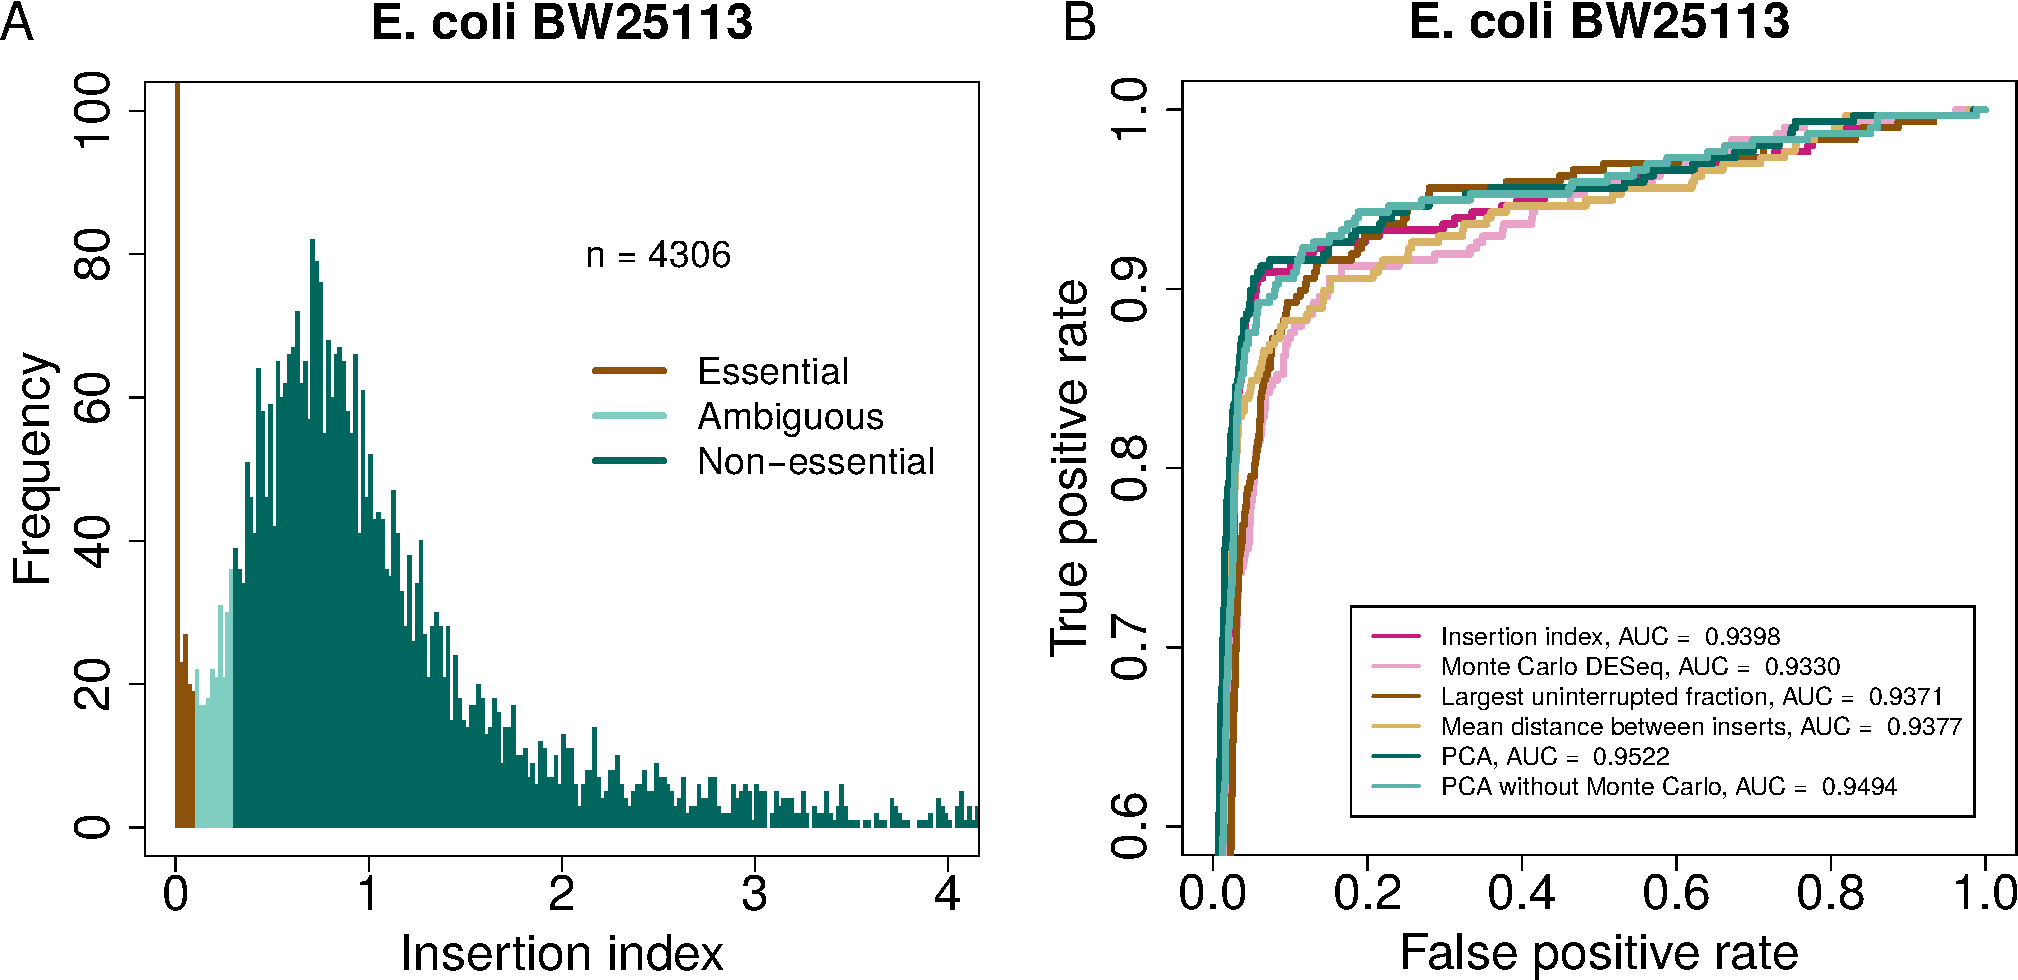
\includegraphics[scale=0.45]{fig1.pdf}
\caption{(a) The bimodal distribution of insertion indices shows different classes of essentiality obtained using DBSCAN. These include essential genes which have the lowest insertion indices, non-essential genes with intermediate insertion indices, beneficial losses with high insertion indices, and ambiguous genes which are located between these groups (b) ROC curves showing the accuracy of 6 methods for predicting essential genes. True positives are genes that are predicted as essential and whose orthologs are essential in EcoGene database of essential genes for \textit{E. coli} K-12 BW25113. False positives are genes that are predicted as essential, but are classed as non-essential in EcoGene study.}
\label{fig:fig1}
\end{figure}

\subsection{What is an ideal insertion density?}
If the number of transposon insertions is too low compared to genome length, the insertion index distribution is not bimodal and therefore the prediction of essential genes is not accurate. However, higher numbers of insertions are labour intensive and cost more due to larger mutant pools which need to be sequenced. Insertion density is defined as the ratio between the number of insertion sites and genome length. In this section, we explore the minimum insertion density which does not affect the accuracy of the experiment.

We provided 4 independent \textit{S.} Typhimurium SL1344 libraries with 50K, 100K, 250K, 500K, and 1000K Colony-Forming Unit (CFU). On average, these libraries have 4075282, 4160203, 4526237, 5711423, and 13813802 reads respectively which results in one insertion site in every 57.07, 52.94, 16.49, 14.17 and 8.86 nucleotides, assuming a uniform distribution of insertions. In order to compare different ranges of insertion densities, we simulated different libraries with one insertion site in 8.86 to 243.90 nucleotides. For each simulated library, we used the closest real library with more insertion sites than our simulated library and randomly omitted insertion sites until we reached the desired density.

The false positive rate declines with the increase of insertion density as illustrated in Figure~\ref{fig:fig2}a and at 0.04 density it becomes almost constant. Figure ~\ref{fig:fig2}b shows that the true positive rate goes down as the insertion density rises to 0.01. This happens due to the large number of predicted essential genes which also includes many actual essential genes. But, as the density increases the number of predicted essential genes decreases which results in a decline in true positive rate. After 0.01, the true positive rate rises with increasing insertion density and it gets almost constant at about 0.04 insertion density. As a result of the fluctuations of the true positive rate and the false positive rate, Matthew's Correlation Coefficient goes up with higher insertion densities until it reaches 0.04. Then, it changes unnoticeably with more insertions (Supplementary Figure 4a). Finally, the percentage of genes with at least 1 insertion rises with higher insertion densities, but the curve becomes almost flat after 0.04 (Supplementary Figure 4b). Overall, these figures show that an insertion density about 0.04 can give us a good trade-off between cost and accuracy.

\begin{figure}[ht]
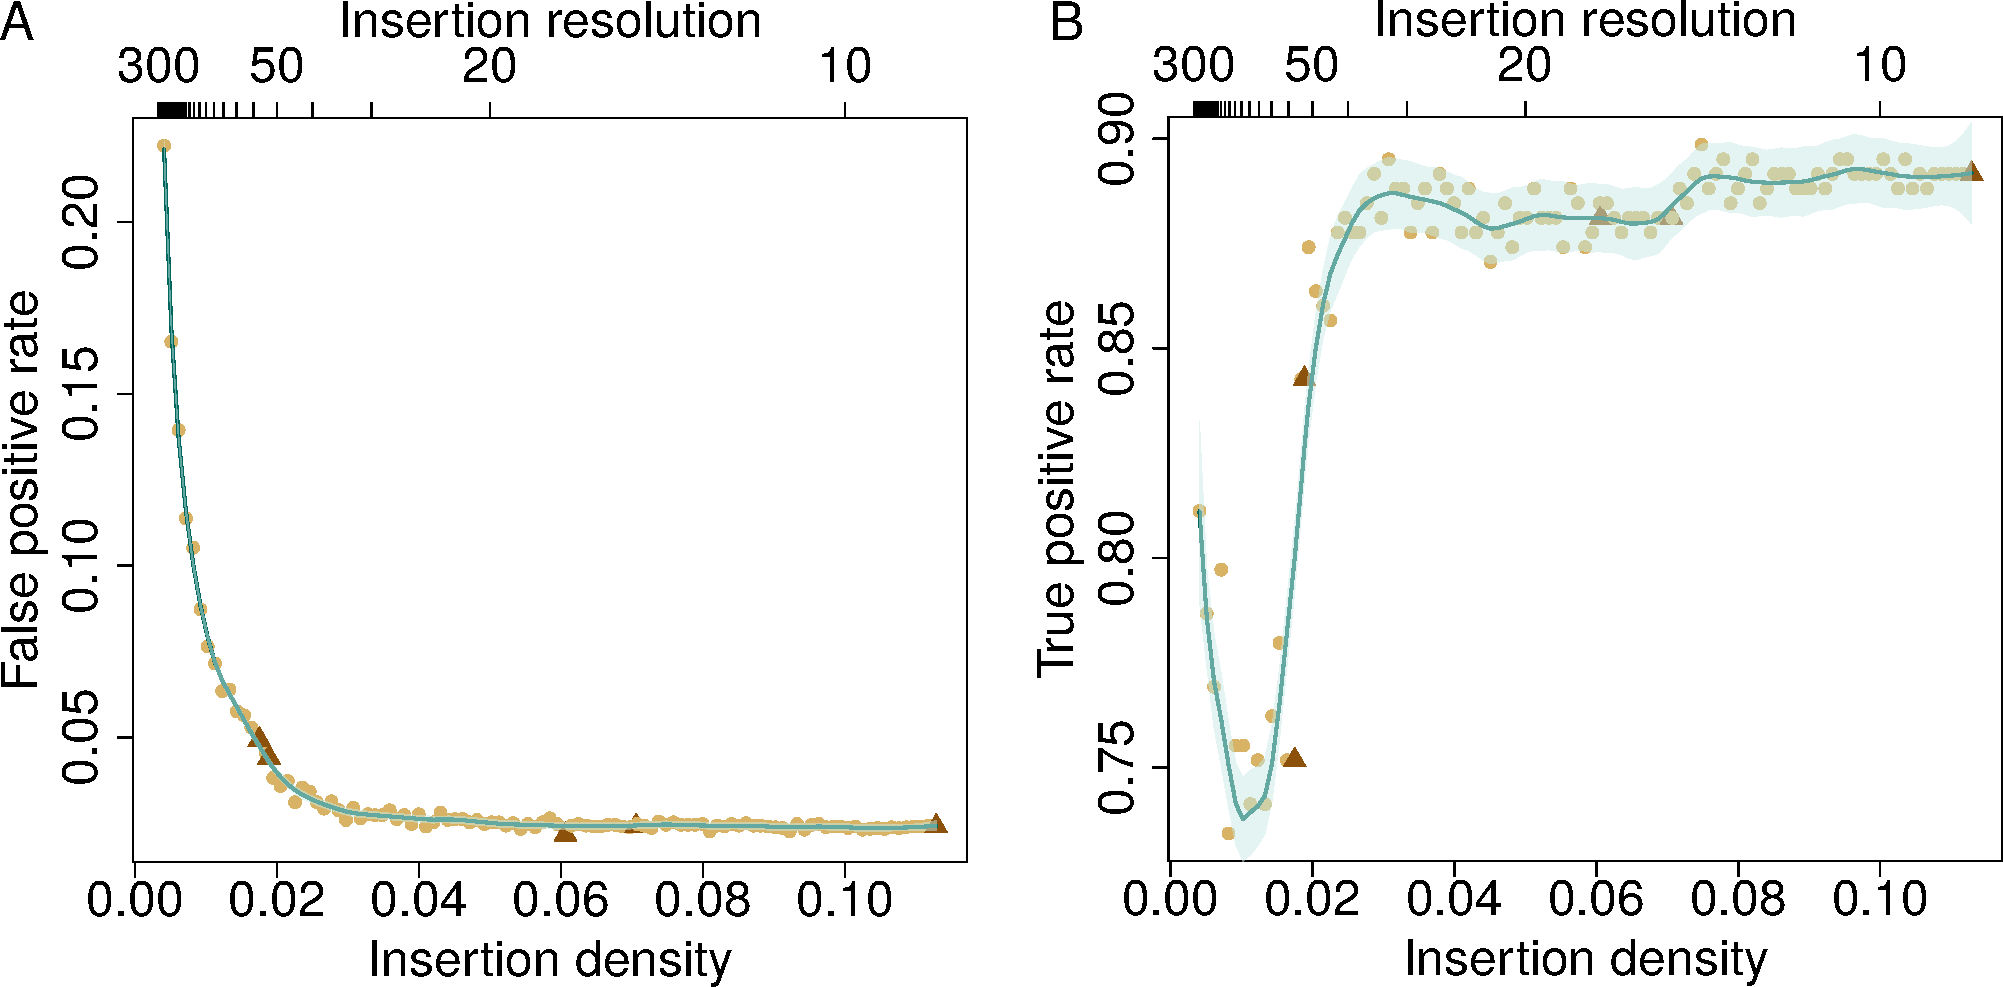
\includegraphics[scale=0.45]{fig2.pdf}
\caption{Simulation of insertion density effects: The red and blue dots are obtained from real and simulated data, respectively. The black line shows the loess curve with 0.2 span and the gray regions show $95\%$ confidence intervals. Insertion resolution is calculated by dividing genome length by the number of insertion sites. (a) False positive rate decreases with the increase of the insertion density (the ratio between the number of insertion sites and genome length) and remains constant after it reaches 0.04. (b) True positive rate goes down as the insertion density rises to 0.01. Afterwards, it rises with increasing insertion density and gets almost constant at about 0.04 insertion density.}
\label{fig:fig2}
\end{figure}

\subsection{Exploring possible sources of bias in TraDIS data}
If the transposon insertion process is biased to specific regions in the genome, it can affect the number of insertions in a gene which changes insertion indices and may put some genes in incorrect essentiality categories. Different articles have reported biases in transposon insertion using Tn5 \cite{goryshin_tn5/is50_1998, langridge_simultaneous_2009, gallagher_genome-scale_2011, canals_high-throughput_2012, green_insertion_2012, zomer_essentials:_2012, barquist_comparison_2013, rubin_essential_2015}. We performed a detailed study of these biases. The biases that we studied include: origin of replication bias, preferred insertion motif bias, and positional bias within genes.

\subsubsection{Distance from the origin of replication bias}
Different studies with conflicting results have been performed on Tn5 insertion bias near the origin of replication \cite{jacobs_comprehensive_2003, gallagher_genome-scale_2011, zomer_essentials:_2012, barquist_comparison_2013, rubin_essential_2015}. When the bacteria are under replication during the transposon insertion process and in the presence of multiple replication forks, there are more copies of the genes close to the origin of replication than the genes further away \cite{barquist_comparison_2013}. To study the insertion bias towards the position of genes within genome, we plotted insertion indices for each gene versus the distance of the gene from the origin of replication normalised by the length of the genome in Figure~\ref{fig:fig3}a. The figure indicates that insertion index decreases when the genes are located further from the origin of replication. This means that there are more insertions in the genes near the origin of replication which can influence the accuracy of our predictions. To correct this bias, we normalised insertion indices by the distance of genes from the origin of replication in genomes (See Methods~\ref{meth:essentiality}).

\subsubsection{Preferred nucleotide composition bias}
Another concern while inferring essentiality from transposon insertion data is that transposon insertion is biased to certain compositions of nucleotides and high number of insertions in genes reflects their enrichment in these motifs, instead of their essentiality level. When Tn5 transposon is inserted into DNA, a region of 9 nucleotides is duplicated on both sides of the transposon \cite{goryshin_tn5/is50_1998}. Some preferred sequence motifs have been proposed previously \cite{goryshin_tn5/is50_1998, canals_high-throughput_2012} which are illustrated in Figure~\ref{fig:fig3}c. Other studies have found no compelling evidence of a preferred insertion motif, but showed the existence of G-C pairs at the two ends of duplicated regions \cite{green_insertion_2012, rubin_essential_2015}. We used Weblogo \cite{crooks_weblogo:_2004} to generate a logo from duplicated regions and 10 nucleotides flanking the 100 top most frequent insertion sites in each genome. The results in Figure~\ref{fig:fig3}c show that the nucleotides in the consensus motifs are just slightly overrepresented compared to the background distribution, however when corrected for background nucleotide composition, there is very little signal (see ``bits'' in Figure~\ref{fig:fig3}c).

The other possible source of bias is if transpositions are more inclined to G-C or A-T rich regions. Rubin et al. \cite{rubin_essential_2015} have reported that the number of Tn5 insertions rises with the increase of G-C content and Green et al. \cite{green_insertion_2012} have shown that the highest number of insertions occurs in the regions in genome with highest G-C content. On the other hand, Langridge et al. \cite{langridge_simultaneous_2009} have seen a high number of Tn5 insertions in between $40\%$ and $50\%$ G-C content and lower number of insertions for G-C content higher than $50\%$. In Figure~\ref{fig:fig3}b, we plotted the G-C content of genes versus their insertion indices for non-essential genes and beneficial losses in a representative genome. The red lines are generalised additive model (GAM) curves with formula $y \sim s(x)$. Insertion indices increase gradually as G-C content rises up to $40\%$-$50\%$ G-C content, after which insertion indices begin to decrease in almost all genomes. In the region where the genes are most densely packed, the GAM curve is almost flat. In \textit{E. coli} BW25113, only 1365 genes have a GC content of less than $50\%$ or greater than $60\%$ which means they are in the region where the density is not flat. On the left side of this flat region, there are genes with different G-C content which are enriched in mobile genetic elements. So, we expect to see more insertions in this region. We have high insertion indices between $40\%$ and $50\%$ G-C content which is expected. However, in most cases when we have less than $40\%$ G-C content, insertion index is low. A possible reason for this phenomena is the association of A-T rich sequences and histone-like nucleotide structuring (H-NS) proteins, which may inhibit the insertions in A-T rich regions. This has been proposed by Barquist et al. for Tn5 \cite{barquist_comparison_2013} and shown for Tn10 transposon \cite{kimura_nucleoid_2016}.

\subsubsection{Positional bias within genes}
Different studies have suggested that transposons are more likely to insert into the ends of a gene compared to the middle \cite{jacobs_comprehensive_2003, hutchison_global_1999, griffin_high-resolution_2011, gallagher_genome-scale_2011, zomer_essentials:_2012}. We have tested this hypothesis using TraDIS data. We divided every gene into 100 fragments with equal lengths (percentiles) and calculated the mean insertion index for each percentile. Insertion indices were calculated using $\frac{n_p/l_p}{n_g/lg}$, where $n_p$ is the number of insertion sites in a specific percentile, $l_p$ is the length of that percentile, $n_g$ is the number of insertion sites in the whole genome and $l_g$ is genome length. Mean insertion index for each percentile is calculated by averaging over all insertion indices for that specific percentile of genes. We observed almost no bias towards any location when considering all genes together (Supplementary Figure 7a). We studied the bias in three different groups of genes: essential genes which have no or just a few insertions, non-essential genes which have an intermediate number of insertions, and beneficial losses which have a high number of insertions. The results imply that the number of insertions in the internal region of the essential genes is outnumbered by the number of insertions in the $5^\prime$ and $3^\prime$ ends (Figure~\ref{fig:fig3}d) while it is the opposite in beneficial losses (Figure~\ref{fig:fig3}e). High number of insertions at the $3^\prime$ end of essential genes implies that the functional domains are located before the insertions and the insertions are not interfering with them. On the other hand, high number of insertions at the $5^\prime$ end of the essential genes indicates there might be alternative start codons in the $5^\prime$ end, or because of annotation errors that have predicted the start codon in an incorrect place before the actual start codon. In our dataset, the number of start codons or alternative start codons (ttg, ctg, or gtg) after insertion sites (in the $5^\prime$-most $10\%$ of the coding sequence) is significantly higher in genes with insertions in their $5^\prime$ end compared to genes without insertions in their $5^\prime$ end (Fisher's exact test P-value = $6.591 \times 10^{-4}$), meaning that alternative start codons and annotation errors are likely to be responsible for high numbers of insertions in the $5^\prime$ end of genes. In order to correct this bias, we trimmed the ends of genes and calculated insertion indices for the remaining parts (see Methods~\ref{meth:essentiality}). 

\begin{figure}
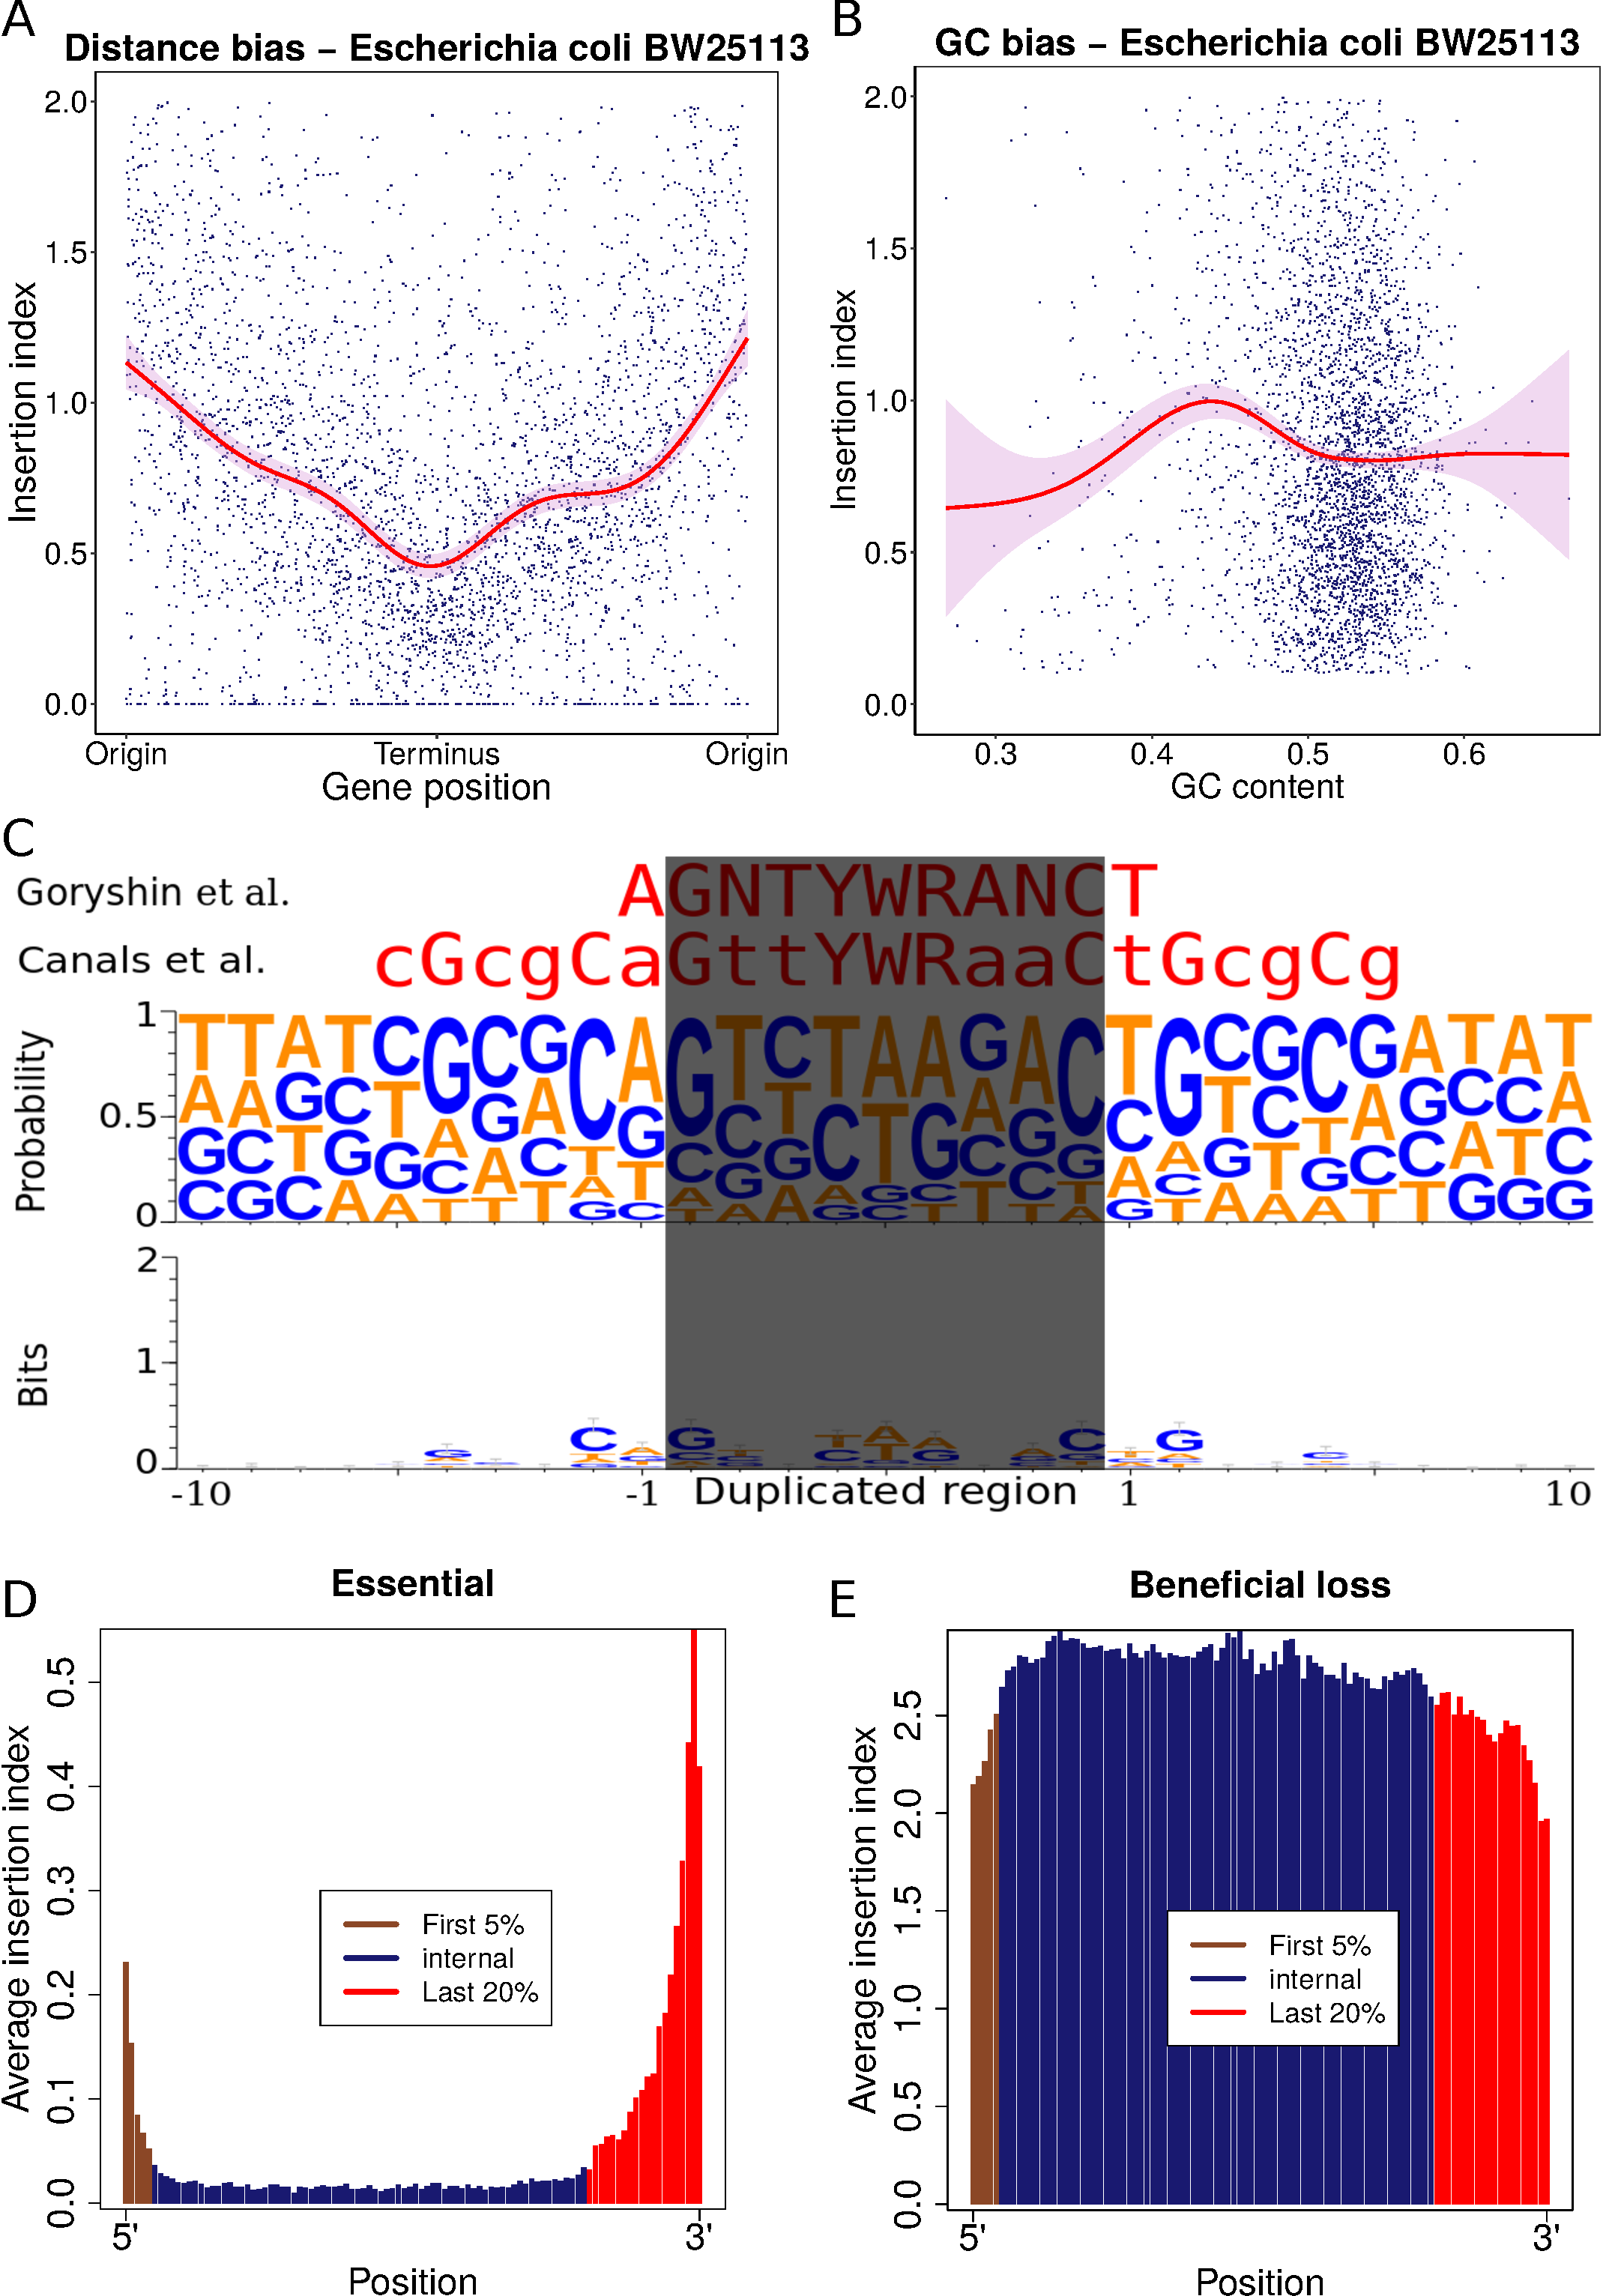
\includegraphics[scale=0.34]{fig3.pdf}
\caption{(a) The distance of \textit{E. coli} genes from the \textit{dnaA} gene (usually found near the origin of replication) versus insertion index. The red line shows the GAM curve when the formula is $y \sim s(x)$ and the pink shading shows $95\%$ confidence interval. (b) G-C content of genes against their insertion indices. The red line shows the GAM curve when the formula is $y \sim s(x)$. (c) Sequence logo plots generated using sequences from the 10 nucleotides flanking the 100 top most frequent insertion sites from each genome. The relative height of each character shows their frequency. (d) and (e) show the average insertion index (mean ii) in percentiles of all essential genes (d) and beneficial losses (e). The genes are divided into 3 segments: $5\%$ of the genes on the $5^\prime$ end, $20\%$ of the genes on the $3^\prime$ end, and the rest in the middle. These are shown by brown, blue, and red respectively.}
\label{fig:fig3}
\end{figure}

\subsection{Essentiality of genes in Enterobacteriaceae}
Previous studies of gene essentiality in representative Enterobacteriales have compared essential genes in different genomes in this family and studied the sets of core essential genes (genes that are conserved in all genomes under study) and accessory essential genes (genes that are conserved in some genomes) \cite{canals_high-throughput_2012, barquist_comparison_2013, freed_combining_2016}. These core essential genes are responsible for essential processes such as cell division, DNA replication, transcription and translation and some important metabolic pathways such as peptidoglycan and fatty acid biosynthesis \cite{barquist_comparison_2013}. Accessory essential genes differ in genomes due to niche adaptation, functional redundancy and the existence of alternative pathways \cite{canals_high-throughput_2012, bergmiller_patterns_2012, barquist_comparison_2013, freed_combining_2016}. Another group of accessory essential genes are phage repressors \cite{barquist_comparison_2013}. Although these genes are not essential for cell growth, once phages are introduced to a cell, they become essential as long as the phage remains in the cell. In this study, we have used transposon insertion coupled with high-throughput sequencing in 13 bacteria from the Enterobacteriaceae family in addition to the list of essential genes in \textit{E. coli} K-12 BW25113 in the EcoGene database \cite{zhou_ecogene_2013} to identify and compare the essentiality of genes in these 14 bacteria, and to identify genes that are essential in all Enterobacteriaceae. Supplementary Figure 8 shows all genes that are essential in at least one bacteria in Enterobacteriaceae and the pathways in which they are involved.
\subsubsection{Core essential genes}
All living organisms need to perform functions that allow them to survive, reproduce, and evolve. Therefore, there is a set of functions that are conserved universally and enable organisms to maintain these essential properties. These functions can be performed by various genes. In this study core essential genes in a clade are defined as genes that are essential in more than $80\%$ of the genomes that we have data for in that clade (Methods~\ref{meth:corecompare}). We have studied core essential genes in different clades in the bacterial evolutionary tree using this dataset, a set of Gammaproteobacteria endosymbionts (Supplementary Figure 11), and the DEG database of essential genes (Supplementary Figure 10). These genes can be helpful to generate a minimal genome. Here, we discuss genes that are essential in different clades which are Enterobacteriaceae, Gammaproteobacteria, Proteobacteria, and all bacteria to see which genes differentiate these clades.

There are 14 core essential genes in all bacteria. These genes are enriched in complexes and pathways related to the ribosome (\textit{rplF}, \textit{rpsC}, \textit{rpsD}, and \textit{rpsE}), aminoacyl-tRNA biosynthesis (\textit{gltx}, \textit{ileS}, \textit{pheS}, and \textit{valS}), and RNA polymerase (\textit{rpoA} and \textit{rpoB}). Other genes in this group are involved in DNA replication (\textit{dnaE}, \textit{gyrB} and \textit{ligA}) and cell division (\textit{ftsZ}). Overall, genes that are essential in all bacteria are involved in replication, transcription, translation, and cell division.

Genes that are core essential in Proteobacteria, but not core essential in all bacteria are enriched in pathways and complexes related to ribosome (\textit{rplE}, \textit{rplK}, \textit{rplM}, \textit{rplO}, \textit{rplP}, \textit{rplQ}, \textit{rplX}, \textit{rpsG}, \textit{rpsK}, and \textit{rpsM}). Although the ribosome is an essential macromolecule, previous studies have shown that not all of the genes in this macromolecule are essential \cite{shoji_systematic_2011, akanuma_inactivation_2012}. Our study shows that a group of genes in ribosome are essential in all bacteria while some others are only essential in some clades, probably due to redundancy or differences in bacteria life-styles. Another pathway enriched in core essential genes in Proteobacteria is terpenoid backbone biosynthesis (\textit{dxr}, \textit{dxs}, and \textit{uppS}). There are two pathways for terpenoid backbone biosynthesis, the mevalonate pathway and the 2C-methyl-D-erythritol 4-phosphate (MEP) pathway. Most of the time only one of these pathways is used \cite{heuston_isoprenoid_2012}, and as a result these genes are not classed as core essential in all groups of bacteria. Similarly, genes that are core essential in Gammaproteobacteria and not core essential in Proteobacteria are enriched in ribosomal genes (\textit{rplB}, \textit{rplL}, \textit{rplN}, \textit{rplR}, \textit{rplT}, \textit{rplV}, \textit{rpmD}, \textit{rpsH}, \textit{rpsL}, \textit{rpsN}, \textit{rpsP}, and \textit{rpsQ}) and terpenoid backbone biosynthesis (\textit{ispE}, \textit{ispF}, \textit{ispG}, and \textit{ispH}) pathways.

Core essential genes in Enterobacteriaceae that are also core in Gammaproteobacteria endosymbionts are enriched in pathways related to riboflavin metabolism (\textit{ribA}, \textit{ribB}, \textit{ribD}, \textit{ribE}, \textit{ribF}, \textit{ribH}), ribosomal genes (\textit{rplC}, \textit{rplD}, \textit{rplJ}, \textit{rplS}, \textit{rplU}, \textit{rplW}, \textit{rpmA}, \textit{rpmB}, \textit{rpsA}, \textit{rpsB}, \textit{rpsJ}, \textit{rpsR}, \textit{rpsS}, and \textit{rpsU}), DNA replication (\textit{dnaB}, \textit{dnaG}, \textit{dnaN}, \textit{dnaX}, \textit{holB}, and \textit{ssb}), peptidoglycan biosynthesis (\textit{ftsI}, \textit{mraY}, \textit{murA}, \textit{murD}, \textit{murE}, \textit{murI}, and \textit{mviN}), and lysine biosynthesis (\textit{asd}, \textit{dapA}, \textit{dapD}, \textit{dapE}, \textit{murE}). Riboflavin metabolism is an essential pathway in bacteria that can be a useful drug target \cite{long_riboflavin_2010}, however the loss of this pathway can be compensated when riboflavin transporters are present and riboflavin is available in the environment \cite{gutierrez-preciado_extensive_2015} which is mostly the case in rich media. Lysine biosynthesis is another essential pathway and drug target \cite{gillner_lysine_2013, hutton_inhibition_2007}. There are three different pathways for this process, the succinylase pathway which is the most common pathway, and the dehydrogenase and acetylase pathways. Some small groups of species (e.g. \textit{Bacillus}) use only the dehydrogenase and acetylase pathways. The existence of lysine in the media and alternative pathways might make genes in this pathway non-essential in some genomes. Lysine biosynthesis feeds into the peptidoglycan biosynthesis pathway, another core essential pathway in this group,  which forms the cell wall. Overall, this group is enriched in genes involved in replication, translation, and cell division.

Finally, genes that are only core essential in Enterobacteriaceae are enriched in pathways related to fatty acid biosynthesis and fatty acid metabolism (\textit{accB}, \textit{accC}, \textit{fabA}, \textit{fabD}, and \textit{fabH}). Although this pathway is essential in gram-negative bacteria, it can be bypassed in gram-positive bacteria as they can incorporate exogenous fatty acids \cite{parsons_identification_2014, parsons_incorporation_2014}. In addition, many of fatty acid related genes might be lost during the reduction of endosymbionts. Supplementary Figure 9 shows the list of genes that are core essential in every clade discussed here.

\subsubsection{Ancestrally essential genes}
As essential genes are responsible for key functions in the cell, it is expected that they are more conserved than  other genes during the evolution of organisms. We have tested this by comparing the number of essential and conserved genes in the common ancestor of our representative \textit{Enterobacter} genomes and in each level in the phylogenetic tree. For this, we used Fitch's algorithm \cite{fitch_toward_1971} to define ancestrally essential and ancestrally conserved genes. The process is explained in Methods~\ref{meth:fitch}. %Table 1 shows which of the genes involved in important biological processes are ancestrally essential.

The phylogenetic tree in Figure~\ref{fig:fig4}a has been annotated with the number of ancestrally essential genes (red) and the number of ancestral genes (blue) at each level. We then plotted the ratios at each level in the phylogenetic tree in Figure~\ref{fig:fig4}b and connected the medians in each level. The connecting line shows that the ratio between ancestrally essential genes and ancestrally conserved genes rises as we go higher in the phylogenetic tree which means essential genes are more likely to be conserved in genomes compared to non-essential genes.

To answer the opposite question, are conserved genes more likely to be essential, we gathered the genes that are conserved in Enterobacteriaceae and defined their conservation level in all bacteria in EMBL database \cite{stoesser_embl_2002} (see: Methods~\ref{meth:conservation}). Figure~\ref{fig:fig4}c shows that conserved genes are more likely to be essential.

\begin{figure}
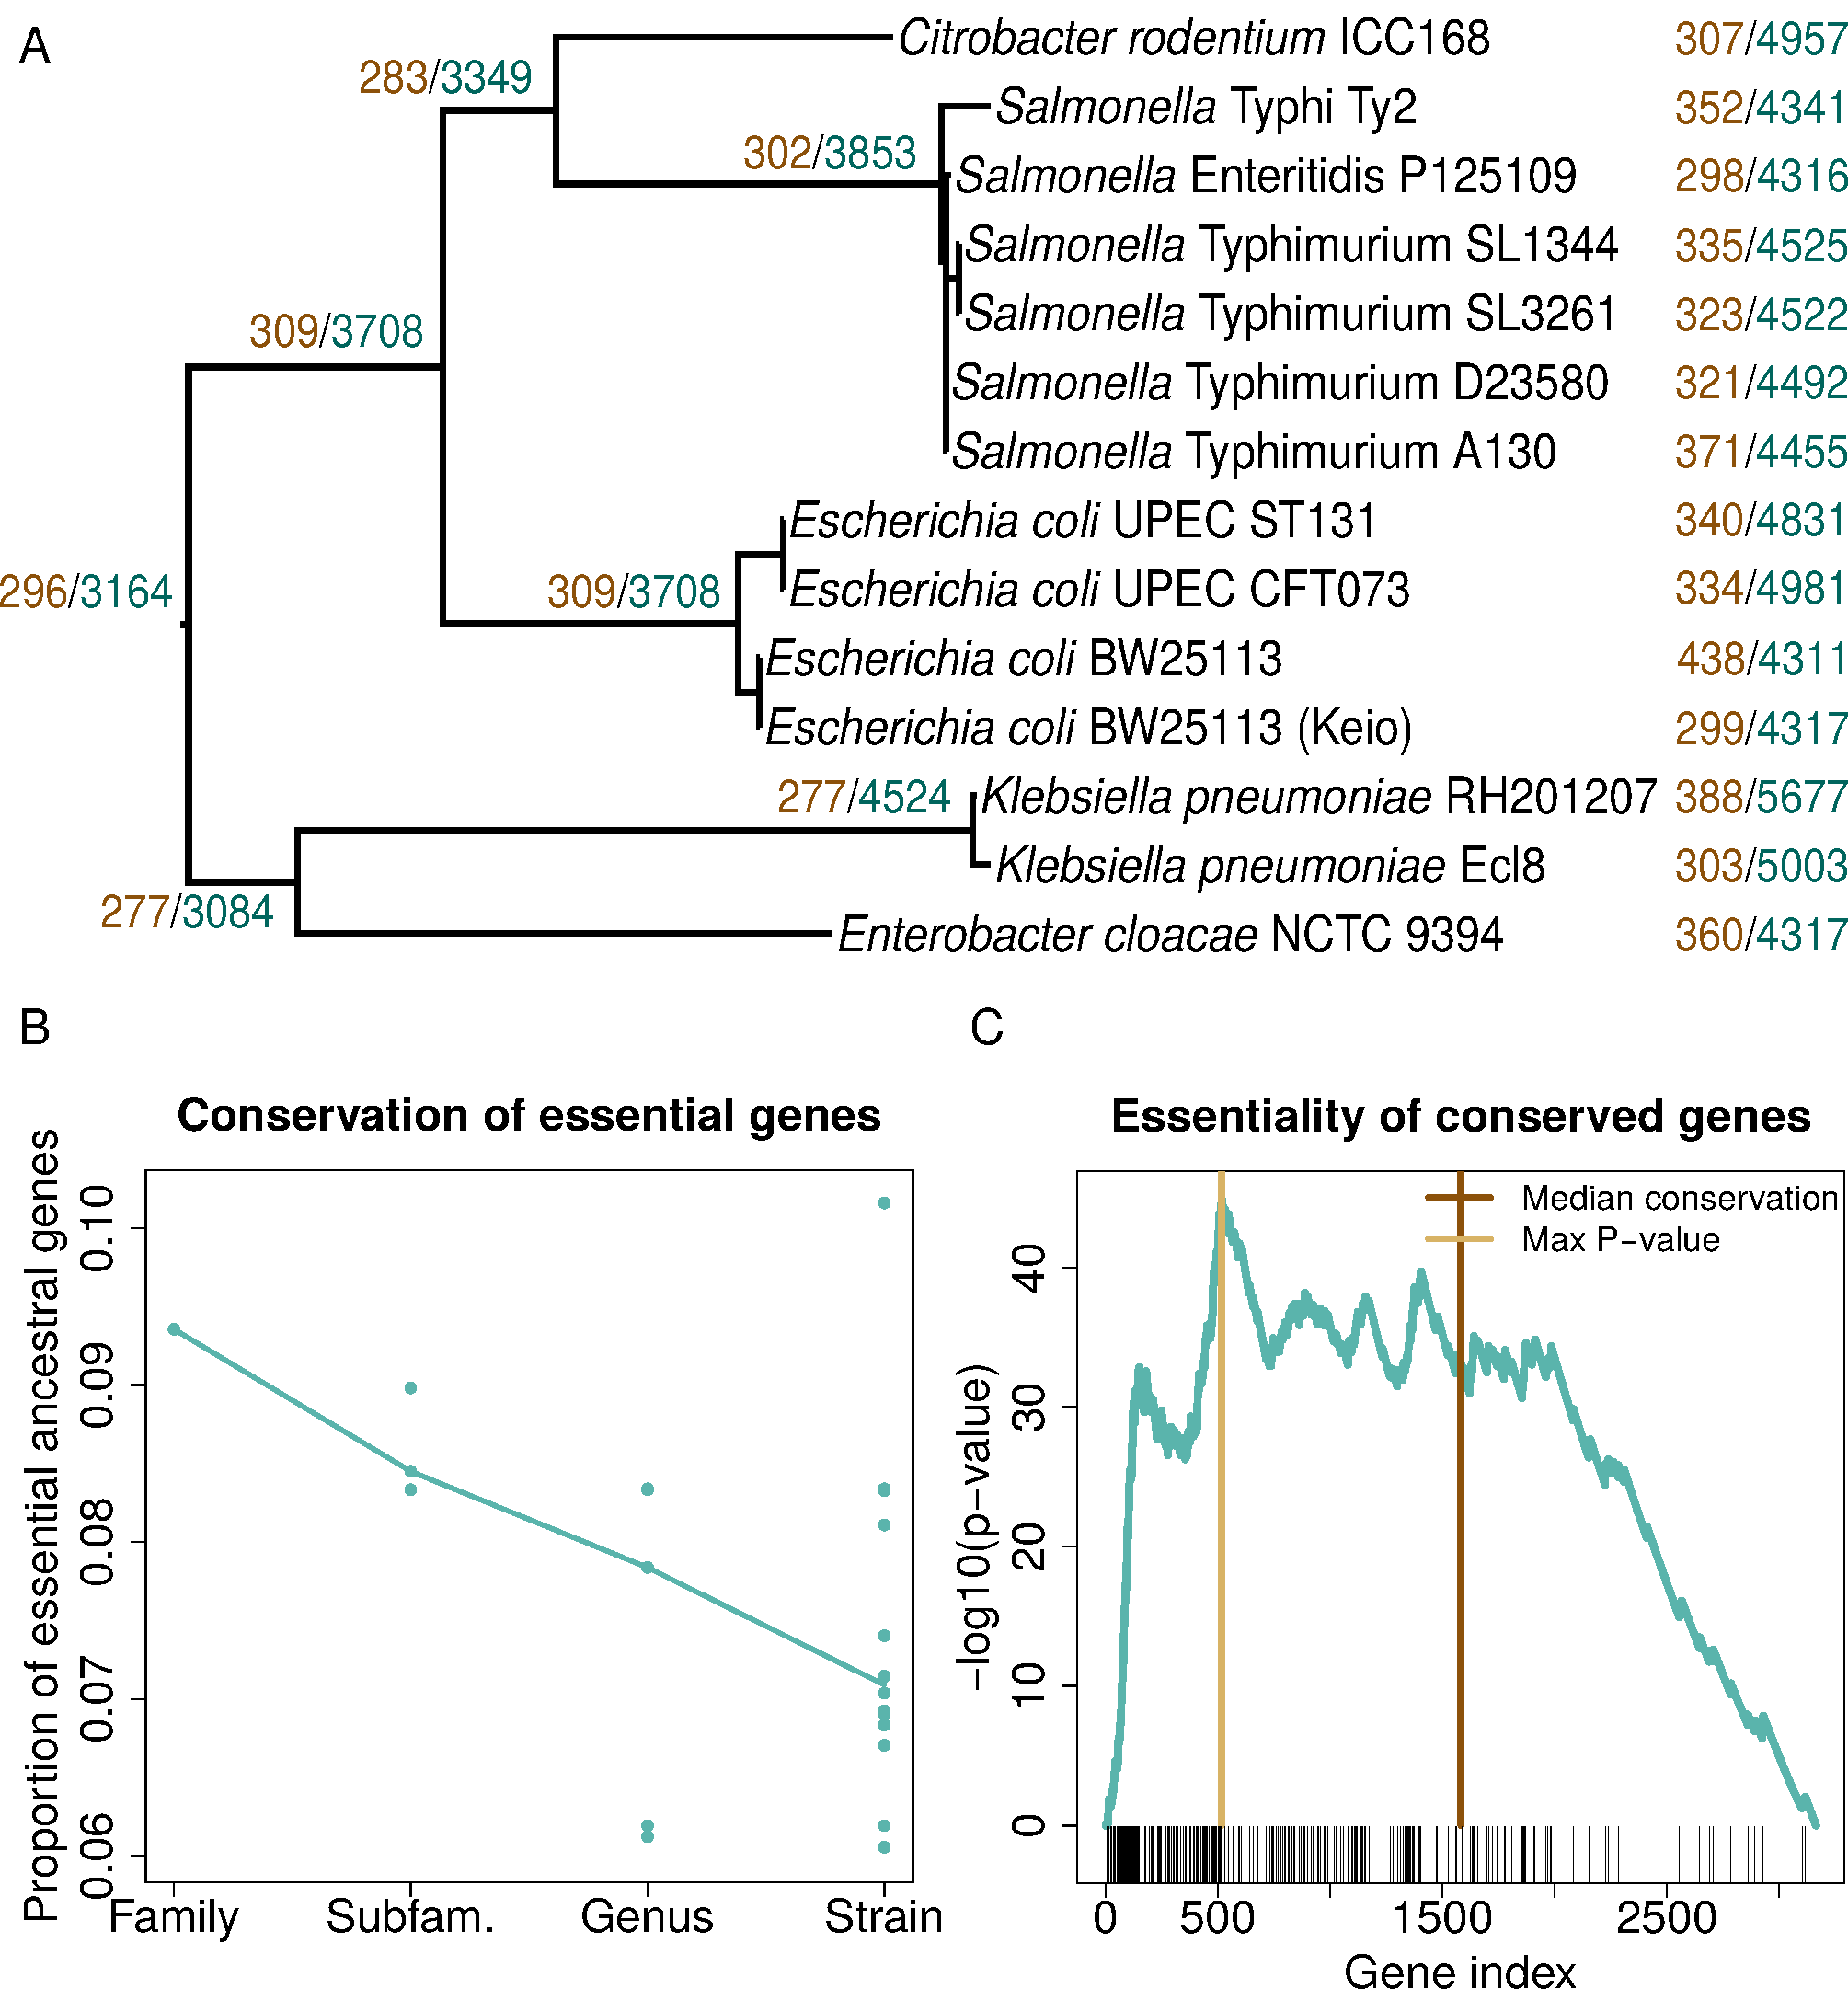
\includegraphics[scale=0.4]{fig4.pdf}
\caption{(a) The species tree for all genomes in this study. Numbers in red show the number of ancestrally essential genes at each level and numbers in blue show the number of ancestral genes at each level. (b) The ratio between ancestrally essential genes and ancestral genes at each level in the species tree. The dots at the strain level show the ratios for all 14 bacteria; the dots at the species level show the ratios for \textit{Enterobacter}, \textit{Klebsiella}, \textit{Citrobacter}, \textit{Salmonella}, and \textit{Escherichia}; the subfamily level shows the ratios for the common ancestor of \textit{Enterobacter} and \textit{Klebsiella}, the common ancestor of \textit{Citrobacter} and \textit{Salmonella}, and the common ancestor of \textit{Citrobacter}, \textit{Salmonella}, and \textit{Escherichia}; and finally the dot in the family level shows the ratio for the root. The line connects the medians in each level. (c) A comparison of essentiality and conservation. Genes conserved in the Enterobacteriaceae family are sorted based on their conservation level in all bacteria from left to right, then a walking hypergeometric test is done from left to right regarding the number of essential genes observed at each step. The khaki line shows the maximum P-value obtained and the blue line shows the gene with median conservation level. Most of the essential genes and the maximum P-value are at the left side of the median showing that conserved genes are more likely to be essential.}
\label{fig:fig4}
\end{figure}

\subsubsection{Accessory essential genes}
Accessory essential genes are important for the design of specialised antibiotics, and can give us insights into the evolution of different genera. Here, we have termed the genes that are ancestrally essential in one genus and not essential in other genera ``accessory essential''. We have used Fitch's algorithm (Materials and Methods) to define ancestrally essential genes in each genus of Enterobacteriaceae for which we had data (\textit{Citrobacter}, \textit{Salmonella}, \textit{Escherichia}, \textit{Klebsiella}, and \textit{Enterobacter}) and studied the genes that are only ancestrally essential in one genus (Supplementary Figure 12). There are five genes that are exclusively essential in \textit{Citrobacter} (\textit{gutQ}, \textit{ihfA}, \textit{ihfB}, \textit{priB}, and \textit{secB}). Among these \textit{ihfA}, \textit{ihfB} and \textit{priB} are related to homologous recombination, \textit{secB} is related to quorum sensing and \textit{gutQ} is arabinose 5-phosphate isomerase. The reason for the essentiality of genes related to homologous recombination might be that \textit{C. rodentium} is a newly evolved and unstable pathogen \cite{petty_citrobacter_2011} and homologous recombination helps with keeping its stability as it can repair DNA damage \cite{darmon_bacterial_2014}.

Ten genes are only ancestrally essential in \textit{Salmonella} which are shown in Supplementary Figure 12. Among these are \textit{fepC}, \textit{fepD}, and \textit{fepG}. \textit{FepB} is also essnetial in 3 out of 6 \textit{Salmonella} genomes in this study, but is not defined as ancestrally essential using Fitch's algorithm. These four genes have been previously shown to be essential in \textit{S.} Typhi and non-essential in \textit{S.} Typhimurium SL1344 \cite{barquist_comparison_2013}. Our analysis shows that they are also essential in \textit{S.} Enteritidis, \textit{S.} Typhimurium D23580, and \textit{S.} Typhimurium A130. This shows the importance of the import of Ferric iron in these genomes. \textit{FtsE} and \textit{ftsX} are other accessory essential genes in \textit{Salmonella}. These genes are ABC transporters that facilitate cell division.%These genes are mostly ABC transporters. As ABC transporters are a large family of genes, some genes in this family might be able to perform the same functions in other genera.

Seven genes are exclusively essential in \textit{Escherichia}. One of these genes is \textit{hipB} which is an antitoxin and is essential in \textit{Escherichia} whenever the toxin (hipA) is present. Another gene in this group is \textit{rpsI} which is 30S ribosomal protein S9. Although this gene has appeared as essential in our study and Keio collection \cite{baba_construction_2006}, it is shown that \textit{E. coli} is viable without this gene despite its slow growth \cite{bubunenko_essentiality_2007, shoji_systematic_2011}. Two other genes in this group are \textit{PhoU} which is a phosphate specific transport system accessory protein whose mutation causes the accumulation of inorganic phosphate in \textit{E. coli} \cite{morohoshi_accumulation_2002} and \textit{crr} which is a component of glucose-specific phosphotransferase enzyme.
%which are involved in different processes and complexes, such as ribosome, quorum sensing, and glycolysis.

The seven genes that are only essential in \textit{Klebsiella} are involved in lipopolysaccharide (LPS) biosynthesis. Bacterial lipopolysaccharides are composed of three components namely, lipid A, core, and O-antigen and core is further divided into two regions, inner core, and outer core \cite{caroff_structure_2003}. These seven essential genes belong to the inner core. LPS is important for stabilising membrane in gram negative bacteria \cite{salton_structure_1996}.
%It has previously been shown that \textit{Klebsiella} produces an extracellular toxic complex that contains LPS \cite{straus_importance_1985, straus_production_1987}. This complex is responsible for the damage to lung tissues which causes pneumonia and its toxicity is associated to LPS \cite{straus_importance_1985, straus_production_1987}. We hypothesise that the importance of this complex and its correlation with the virulence of \textit{Klebsiella} \cite{domenico_extracellular_1985} is the reason for the essentiality of 7 LPS related genes specifically in \textit{Klebsiella}. 
 
%and finally, the 22 genes that are only essential in Enterobacter are involved in different functions e.g. streptomycin biosynthesis, sulfur relay system, and aminoacyl-tRNA biosynthesis.
Finally, the 22 genes that are only essential in \textit{Enterobacter} are involved in different functions e.g. sulfur relay system and aminoacyl-tRNA biosynthesis. Further studies are needed to find out the reason for the essentiality of these genes in \textit{Enterobacter}. Moreover, as the \textit{Enterobacter} genus contains only one genome in our dataset, the essentiality of these genes should be studied on different species in this genus.

\subsubsection{Genus-specific, conserved single-copy and conserved multi-copy genes}
To study the relationship between copy number and essentiality of genes, we divided the genes in this study into 3 groups: genus-specific genes that are present only in one genus, conserved single-copy genes that are present once almost in all genomes in our study, and conserved multi-copy genes that are conserved and have multiple copies in each genome. The procedure for defining these three groups is described in Methods~\ref{meth:homclust}. The distribution of each class is depicted in Figure~\ref{fig:fig5}.

The high number of conserved single-copy essential clusters (380 single-copy essential clusters out of a total of 612 essential clusters), indicates that there is a set of essential genes in Enterobacteriaceae that are conserved and remained essential. However, there are also many essential genus-specific genes (214 genus-specific essential clusters). Most of the conserved multi-copy clusters are non-essential according to TraDIS. This can be explained by the redundancy of function that duplicate genes can retain even after long divergence times \cite{dean_pervasive_2008} which allows duplicates of knocked-out genes to compensate. Therefore, if a gene is essential and has multiple copies in the genome, transposon insertion sequencing is generally unable to detect its essentiality.

Figure~\ref{fig:fig5} also shows that beneficial losses are over represented in the genus-specific class. Therefore, beneficial losses are mostly newer genes that are deleted or mutate over time. Moreover, the figure shows that conserved multi-copy genes have few clusters tagged as beneficial loss, meaning that beneficial losses are less likely to have multiple copies in an organism. We tested whether the reason for this phenomenon is that beneficial losses are copied on plasmid which causes these genes have fewer copies due to high cellular copy number. For this, we compared the number of clusters tagged as beneficial loss that had at least one homolog on plasmids of the genomes in this study, the number of clusters tagged as beneficial loss with no homologs on plasmids, the number of clusters that are not grouped as beneficial loss with at least one homolog on plasmids, and the number of clusters that are not grouped as beneficial loss with no homologs on plasmids using Fisher's exact test. The resulting P-value is 0.31 which shows no statistically significant difference between copies of genes on plasmids in beneficial loss group and others.

As beneficial losses are mostly genus specific, there is not much information about them and most of them do not exist in databases like KEGG and GO. Therefore, in order to investigate beneficial losses we studied the words that were enriched in the description of gene product in EMBL files. The list of enriched words is provided in Supplementary Table 1. The table shows that beneficial losses are mostly mobile genetic elements (e.g. transposable elements, pathogenicity islands, and bacteriophages), putative or hypothetical proteins, and bacterial adhesins (e.g. fimbria, curli, and pilin). Mobile elements are newly acquired genes, so the organism does not generally require them. Bacterial adhesins help the bacteria to adhere together and colonise. Even though these genes are required when the bacteria are living in their host, they are not essential in rich media.

\begin{figure}
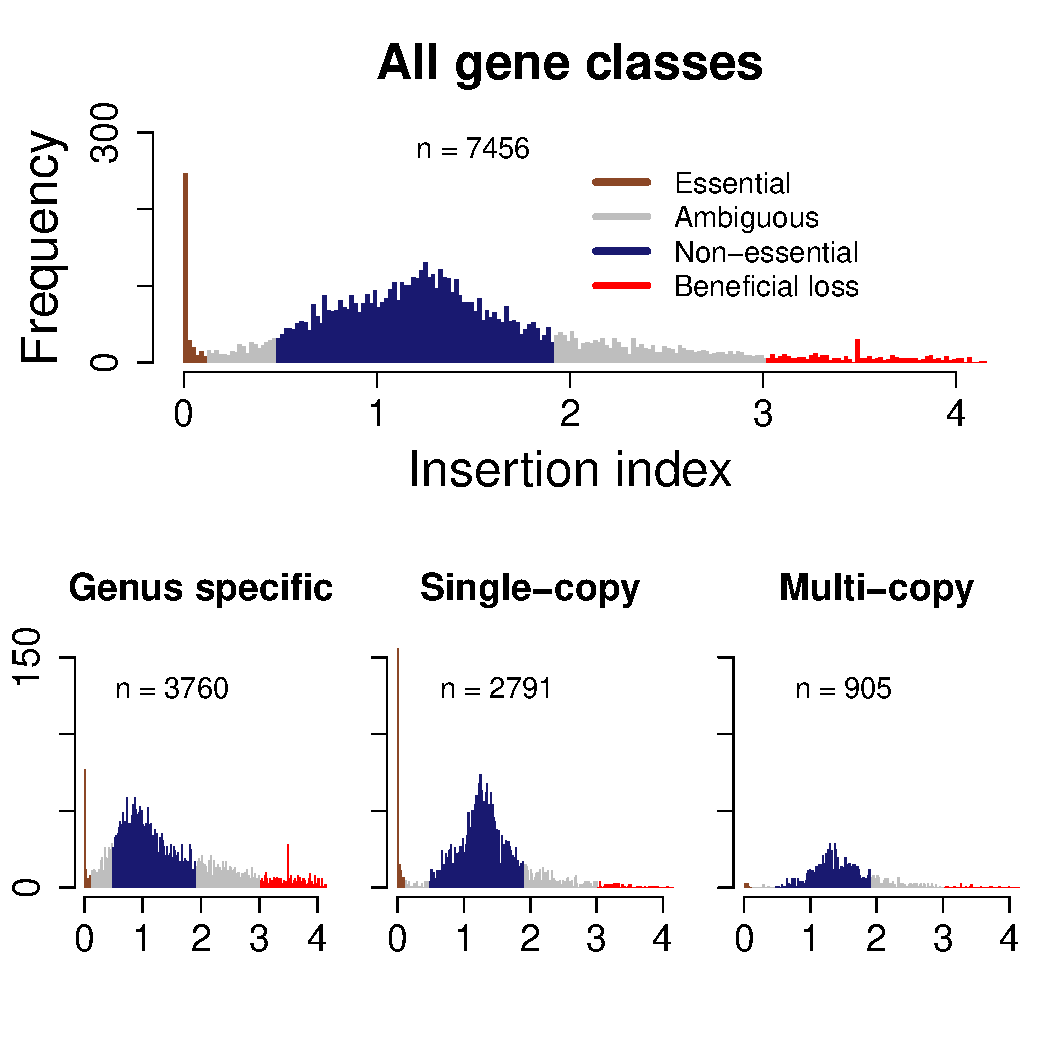
\includegraphics[scale=0.8]{fig5.pdf}
\caption{Genes clustered into homologous groups using Jackhmmer and divided into 3 groups: genus-specific, conserved single-copy, and conserved multi-copy genes. The essentiality of the clusters has been defined using the insertion indices of the genes in the clusters.}
\label{fig:fig5}
\end{figure}

\section{Conclusion}
Our analysis shows what is needed in order to accurately identify essential genes in a transposon insertion experiment. Transposon insertion density is a major factor for the accuracy of this experiment. Our study shows that on average having one insertion site in every 25 nucleotides can accurately differentiate between essential and non-essential genes. When transposon insertion sequencing is performed, a measure is needed for distinguishing between essential and non-essential genes. Despite its simplicity, insertion index has high accuracy and can quickly evaluate the essentiality of a gene. However, there are biases that can affect the accuracy of this method. We studied different biases and showed that the distance from the origin of replication can affect the number of insertions observed in a gene. To overcome this bias, we normalised insertion indices by the distance of genes from the origin of replication in genomes. In addition, the two ends of genes do not have insertion patterns similar to the intermediate region. Therefore, we calculated insertion indices after trimming the ends.

This study shows the sets of essential genes in 14 bacteria from Enterobacteriaceae and shows that these genes are involved in pathways related to replication, transcription, translation, and protein export. Other enriched pathways are predominantly involved in metabolic processes. These include fatty acid biosynthesis that produces cell membrane, peptidoglycan and lipopolysaccharide biosynthesis that are essential components of cell wall, terpenoid backbone biosynthesis which feeds peptidoglycan biosynthesis, nucleotide and amino acid metabolism, and the metabolism of important cofactors and vitamins like riboflavin, biotin, and porphyrin.

Moreover, we studied the accessory essential genes in each genus of Enterobacteriaceae and showed that the genes that are exclusively essential in each genus help with the specific lifestyle of the genomes in that group. Genes related to homologous recombination are essential in \textit{Citrobacter}. The reason might be that they reduce genome instability by repairing DNA damage \cite{darmon_bacterial_2014}. In addition, genes related to LPS, which help with membrane stability \cite{salton_structure_1996}, are essential in \textit{Klebsiella}. The essential genes in \textit{Salmonella} are mostly related to the import of Ferric iron.

The comparison of the essential genes in Enterobacteriaceae with the essential genes in Gammaproteobacteria, Proteobacteria, and all bacteria shows that many genes are not essential in all groups because of the existence of other genes and pathways that compensate for them. The genes that are essential in all bacteria are involved in ribosome complex, aminoacyl-tRNA biosynthesis, RNA polymerase, DNA replication, and replication. Some genes in terpenoid backbone biosynthesis pathway are not essential in all bacteria but core essential in Proteobacteria or Gammaproteobacteria. The reason might be that, even though terpenoid backbone biosynthesis is an important pathway for the formation of cell wall, there are two pathways for this process, most of the time only one of which is used in a genome \cite{heuston_isoprenoid_2012}. There are genes related to lysine biosynthesis that are core essential in Enterobacteriaceae and core in Gammaproteobacteria endosymbionts, but not core essential in all bacteria. These genes are related to the production of diaminopimelate (DAP) which is important in cell wall biosynthesis. The reason these genes are not core essential in all genomes might be the presence of lysine in the media and alternative pathways. Finally, many fatty acid biosynthesis genes are only core essential in Enterobacteriaceae. This pathway is only essential in gram negative bacteria \cite{parsons_identification_2014, parsons_incorporation_2014}.
%Moreover, we studied the essential genes in each genus of Enterobacteriaceae family and showed that the genes that are exclusively essential in each genus help with the specific lifestyle of the genomes in that group e.g. by reducing genome instability, and increasing virulence of organisms. %Moreover, genes related to fatty acid metabolism and biosynthesis pathways are only core essential in Enterobacteriaceae. Bacterial type II fatty acid synthesis (FASII) is one of the targets for antibacterial agents \cite{yao_how_2015, freiberg_novel_2006, schiebel_rational_2014}. Although this pathway is essential in gram-negative bacteria, it can be bypassed in gram-positive bacteria as they can incorporate exogenous fatty acids \cite{parsons_identification_2014, parsons_incorporation_2014}. The FASII cycle involves Acetyl-CoA carboxylase (accABCD), and fatty acid biosynthesis genes (fabABDFGHIKLVZ) of which accABCD, fabH, fabI, and fabBF have been targeted by antibacterials \cite{yao_how_2015}. AccB, accC, and fabH are only core essential in Enterobacteriaceae, while accA and accD are core essential in Enterobacteriaceae and Gammaproteobacteria. However, these genes are not core in endosymbionts which might be because they can provide their needed fatty acid from their host. fabI and fabB are core essential in Enterobacteriaceae and endosymbionts and fabF is not core essential anywhere.

The comparison of conservation and essentiality of genes shows that essential genes are less likely to be lost over time compared to non-essential genes. The reverse applies as well; genes that are conserved are more likely to be essential. Our analyses also show that essential genes identified using transposon insertion sequencing include genes that are conserved in all Enterobacteriaceae, or exclusive to single strains. But very few conserved multi-copy genes are essential since the other copy can compensate for the knocked out gene. Finally, most of the genes that an organism tends to lose are genus-specific. We also showed that genes that are beneficial to lose in a rich medium are mostly related to mobile genetic elements or bacterial adhesion.

\section{Materials and methods}
In this section we will firstly discuss how the essentiality of genes in 13 bacteria from Enterobacteriaceae were evaluated. Secondly, we will explain the methods used to cluster orthologous and homologous genes. Afterwards, the ancestrally essential and ancestral genes are defined. Subsequently, we will explain how core genes are defined in our dataset of 14 bacteria from the Enterobacteriaceae family, DEG database, and our dataset of endosymbionts. In addition, the process for calculating conservation levels of genes is described and finally we will describe the method used for pathway enrichment analysis.

\subsection{Identifying essential genes}\label{meth:essentiality}
In order to find essential genes for this study, we require a metric to evaluate if a gene is essential or not. For this, we used insertion index as it is an accurate and simple predictor of gene essentiality (Figure~\ref{fig:fig1}a). The insertion index for each gene in each genome is calculated using $\frac{n_g/l_g}{n_o/l_o}$ where $n_g$ is the number of insertion sites in the gene after trimming $5\%$ from the $5^\prime$ end and $20\%$ from the $3^\prime$ end (because the regions close to the $5^\prime$ and $3^\prime$ ends are tolerant of insertions, even in essential genes as shown in Figure~\ref{fig:fig3}d), $l_g$ is the length of the gene after cutting $5\%$ from the $5^\prime$ end and $20\%$ from the $3^\prime$ end, $n_o$ is the number of insertion sites in the genome, and $l_o$ is the length of the genome. Since the insertion of transposons is biased towards the distance from origin of replication, we should normalise insertion indices. In each genome, we fitted a GAM curve when the formula is $y \sim s(x)$ to the distance vs. insertion index plot using R. Then, we calculated the distance-normalised insertion indices by dividing insertion indices by predicted values using the GAM curve and then multiplying them to average insertion index.

We used DBSCAN R package \cite{ester_density-based_1996} and clustered the normalised insertion indices using DBSCAN function with parameters minPts = 200 and eps = 0.05. DBSCAN groups all the genes whose distance from each other is less than or equal to eps. If the number of genes in each group is greater than or equal to minPts, these genes are in one cluster and otherwise, they are identified as noise. This algorithm finds two clusters which are essential genes and non-essential genes shown by brown and blue in Figure~\ref{fig:fig1}a, respectively. The noise data is scattered in two regions; between essential and non-essential clusters and on the right side of non-essential genes. These are shown by both gray and red in Figure~\ref{fig:fig1}a. The noises between essential and non-essential genes were termed ambiguous. Since the noises in the right side of the plot involved some parts of the second peak in insertion index distribution (the rightmost gray region in Figure~\ref{fig:fig1}a) and the long tail on the right (the red region in Figure~\ref{fig:fig1}a), we separated these two regions and called the genes in the right side of the plot beneficial losses. For this, we reran DBSCAN on the group of genes with high insertion index with minPts = 100 and eps = 1. This gives us a cluster of genes that are between the non-essential genes and the long tail of the insertion index distribution. The genes in this cluster are called ambiguous and the rest of the genes on the right side of this ambiguous region are beneficial losses.

\subsection{Genus-specific, conserved single-copy and conserved multi-copy genes}\label{meth:homclust}
In order to test if copy number can affect the essentiality of genes identified using transposon insertion sequencing, we studied the essentiality of genes in three groups, genus-specific, conserved single-copy, and conserved multi-copy genes. For this we needed to cluster homologs (both orthologs and paralogs). We developed a homologous protein clustering methods (HomClust) using Jackhmmer from HMMER package \cite{eddy_accelerated_2011} and clustered genes based on Jackhmmer results. This program iteratively searches for homologous proteins in a dataset. We first used Jackhmmer with 5 iterations, E-value threshold set to $10^{-10}$, and MSV threshold (F1) equal to $10^{-3}$ to find all genes in all genomes that were homologous to \textit{C. rodentium} genes. Other parameters used in Jackhmmer were the default parameters. Then, we selected genes that were not clustered in the first step and reran Jackhmmer with the same parameters to compare these genes with all genes and cluster them. If the length of the homologous domain was less than $80\%$ of the length of the gene itself, we omitted that gene from the cluster.

The above clustering, results in some very large clusters (e.g. ABC transporters, transcriptional regulators, and dehydrogenases), which can be divided into closer groupings. We collected the clusters that had more than 48 members and reran Jackhmmer on them with 1 iteration and more stringent thresholds, $10^{-20}$ E-value threshold and $10^{-6}$ MSV threshold. Then, we collected all the clusters with less than 5 members and generated a dataset that contains the members of these clusters. We reran Jackhmmer on this dataset with more permissive parameters which is 5 iterations, $10^{-5}$ E-value threshold, $10^{-3/2}$ MSV threshold, and $10^{-3/2}$ inclusion E-value threshold (the default value for inclusion E-value threshold which was used in previous steps is $10^{-3}$). Jackhmmer produces multiple local alignments on the same genes resulting in clusters containing whole genes as well as shorter segments within genes. In order to solve this problem, merged the members of clusters in case they had more than $80\%$ overlap. Finally, clusters with more than $80\%$ sequences in common got merged.

In order to study the essentiality of different classes of genes, we divided the clusters of homologous genes into three classes based on their conservation and copy number; genus-specific class, conserved single-copy class, and conserved multi-copy class. The genus-specific class contains clusters that include genes that are present only in one genus. In order to separate conserved single-copy from conserved multi-copy genes, we define a threshold of $70\%$. %If a single gene is duplicated in 2 of 12 genomes, should that cluster be called conserved single-copy or conserved multi-copy? In order to solve this problem, we called clusters conserved single-copy if a minority of genes in them were duplicated. For this, we used a $70\%$ threshold.
The genes in the conserved single-copy class are present in more than one genus and more than $70\%$ of them are not duplicated, while the genes in conserved multi-copy class are present in more than one genus and more than $30\%$ of them are duplicated (duplicate genes).

\subsection{Clustering orthologous sequences}\label{meth:ortholog}
To compare the essentiality of genes in different organisms, we needed to cluster orthologous genes. For this purpose, we used Hieranoid \cite{schreiber_hieranoid:_2013} with default parameters. Clustering with Hieranoid can be performed either using BLAST \cite{altschul_basic_1990, altschul_gapped_1997} or USEARCH \cite{edgar_search_2010}. We used BLAST as Hieranoid's similarity search tool. Hieranoid needs a species tree for clustering. To generate the species tree, we first ran PhyloSift-search on all the genome sequences to find the orthologs of marker genes in PhyloSift database \cite{darling_phylosift:_2014}. Subsequently, we ran PhyloSift-align to align the genes found in previous step. Finally, we concatenated the alignments and ran RaXMLHPC \cite{stamatakis_raxml_2014} to generate a tree. The parameters used for these tools are listed in Table \ref{tab:param}.

\begin{table}[]
\caption{Tools used for generating the species tree for genomes used in this study and their parameters}
\label{tab:param}
\begin{tabular}{ll}
\textbf{Tool} & \textbf{Parameters}\\
\hline
\hline
PhyloSift-search & isolate \\
 & besthit \\
\hline
PhyloSift-align & isolate \\
 & besthit \\
\hline
RaXMLHPC & m PROTGAMMALG4M \\
 & f a \\
 & $\#$ 100\\
\end{tabular}
\end{table}

\subsection{Defining ancestrally essential and ancestrally conserved genes}\label{meth:fitch}
In order to compare the number of genes that are essential at each level in the phylogenetic tree with the number of genes that are conserved, we used Fitch's algorithm \cite{fitch_toward_1971} with a binary alphabet on both essentiality (0 for non-essential and 1 for essential) and conservation (1 for the presence and 0 for the absence of genes). The Fitch's algorithm defines the status of each node in the tree by finding the order that minimises the number of mutations. Here, mutations are changes in essentiality or the conservation of genes. Therefore, by using Fitch's algorithm on gene essentiality, we minimise the number of times a gene has lost or gained essentiality during evolution assuming that this process is rare. Likewise, by using this algorithm on gene conservation, we minimise the number of times a gene has been lost or gained throughout time. Here, we describe how we used Fitch's algorithm for defining ancestrally essential genes. Defining ancestrally conserved genes is the same.

For every gene, considering the phylogenetic tree of the genomes in this study, we assigned a set that contains only one member to each leaf of the tree. If the desired gene was essential in the genome at each leaf, the assigned set contained zero, and if the gene was not essential, the set contained one. The parent of every two nodes was labelled with the intersection of its children's assigned sets, if the intersection was not empty. Otherwise, it was labelled with the union of its children's assigned sets. We continued this process until we reached the root of the tree. At the root, if the assigned set only contained 1, the gene was considered ancestrally essential. Otherwise, it was considered ancestrally non-essential.

\subsection{Comparison of core essential genes in Enterobacteriaceae, endosymbionts, and DEG database}\label{meth:corecompare}
In order to see how essentiality of genes has changed during evolution, we compared core essential genes at different levels of bacterial phylogeny which includes Enterobacteriaceae, endosymbionts, Gammaproteobacteria, Proteobacteria, and all bacteria. The data for essentiality of genes in Enterobacteriaceae comes from the 14 genomes in our study and the data for other groups excluding endosymbionts is obtained from DEG database \cite{luo_deg_2014}. We only included data from studies that were performed in a rich medium. For some genomes there were multiple studies of essential genes. There were two studies on \textit{E. coli} BW25113 in DEG \cite{gerdes_experimental_2003, baba_construction_2006}, from which we only included the Keio collection \cite{baba_construction_2006} as it uses single gene knockout and is considered to be high accuracy. %Among the three studies on \textit{Mycobacterium tuberculosis} H37Rv \cite{sassetti_genes_2003, griffin_high-resolution_2011, zhang_global_2012} which were either using transposon mutagenesis coupled with high-throughput sequencing or transposon site hybridization, we used the most recent one which uses transposon mutagenesis along with high-throughput sequencing \cite{zhang_global_2012}. Likewise, among the two studies on \textit{Porphyromonas gingivalis} ATCC 33277 that used similar methods \cite{klein_identification_2012, hutcherson_comparison_2016}, we selected the most recent one \cite{hutcherson_comparison_2016}. Finally, there were two studies on \textit{Pseudomonas aeruginosa} PAO1 using Tn-Seq \cite{gallagher_genome-scale_2011, turner_essential_2015}, among which we only used the most recent one \cite{turner_essential_2015}.
When multiple studies have investigated the essentiality of genes of the same organism, the most recent one was favoured (i.e. \cite{zhang_global_2012, hutcherson_comparison_2016, turner_essential_2015}). Supplementary Figure 10 shows all the genomes and studies from which the essential genes were identified. The orthologous genes are found using Hieranoid as explained in Section~\ref{meth:ortholog}.

Endosymbionts were selected from Gammaproteobacteria. Supplementary Figure 11 shows all of the endosymbionts in this study. We have included endosymbionts since they have extremely reduced genomes, that have lost many non-essential genes. To define core essential genes in each sub-clade, we have calculated the ratio between the number of genomes in which the gene is essential in the sub-clade and the number of all genomes in the sub-clade. The gene was considered core essential if this ratio is greater than 0.8.

\subsection{Defining the conservation level of gene clusters}\label{meth:conservation}
For the study of the relationship between conservation and essentiality, we defined the conservation level of each gene as below.

To define the distance between every pair of bacteria, we used cmsearch from infernal package \cite{nawrocki_infernal_2013} to find the best hit to 16S rRNA (RF00177 Rfam CM model) in each bacterial genome in EMBL database \cite{stoesser_embl_2002} downloaded at 14/4/2016 and then aligned these sequences to the 16S model using cmalign from Infernal. Subsequently, a distance matrix was generated using dnadist from the PHYLIP package \cite{felsenstein_phylip-phylogeny_1989} and the F84 model that defines the distances.  Afterwards, we gathered all 3164 gene clusters that are ancestrally conserved in Enterobacteriaceae and generated HMM profiles for each of these clusters using HMMER \cite{eddy_accelerated_2011}. The resulting HMM profiles were compared to the genes in all bacterial genomes in EMBL and the maximum distance between all hits was used as the conservation level for each gene.

\subsection{Pathway enrichment analysis}
We used KEGG \cite{kanehisa_kegg:_2000} pathway enrichment analysis to study different groups of genes and their functions. Only pathways for \textit{C. rodentium} ICC168, \textit{S.} Typhi Ty2, \textit{S.} Enteritidis P125109, \textit{S.} Typhimurium SL1344, \textit{S.} Typhimurium D23580, \textit{E. coli} UPEC CFT073, \textit{E. coli} K-12 BW25113 from Keio collection, and \textit{E. cloacae} NCTC 9394 genomes were available in KEGG database. The available pathways were downloaded using the KEGGREST package in R and then the pathways related to the desired groups of genes were compared to all pathways using Fisher's exact test. We adjusted the obtained P-values using the Benjamini, Hochberg, and Yekutieli method. Pathways with corrected P-values over 0.05 were considered to be enriched.
%----------------------------------------------------------------------------------------
%	BIBLIOGRAPHY
%----------------------------------------------------------------------------------------
\newpage
\bibliographystyle{apalike}
%\bibliographystyle{natbib}
\bibliography{refs2.bib}

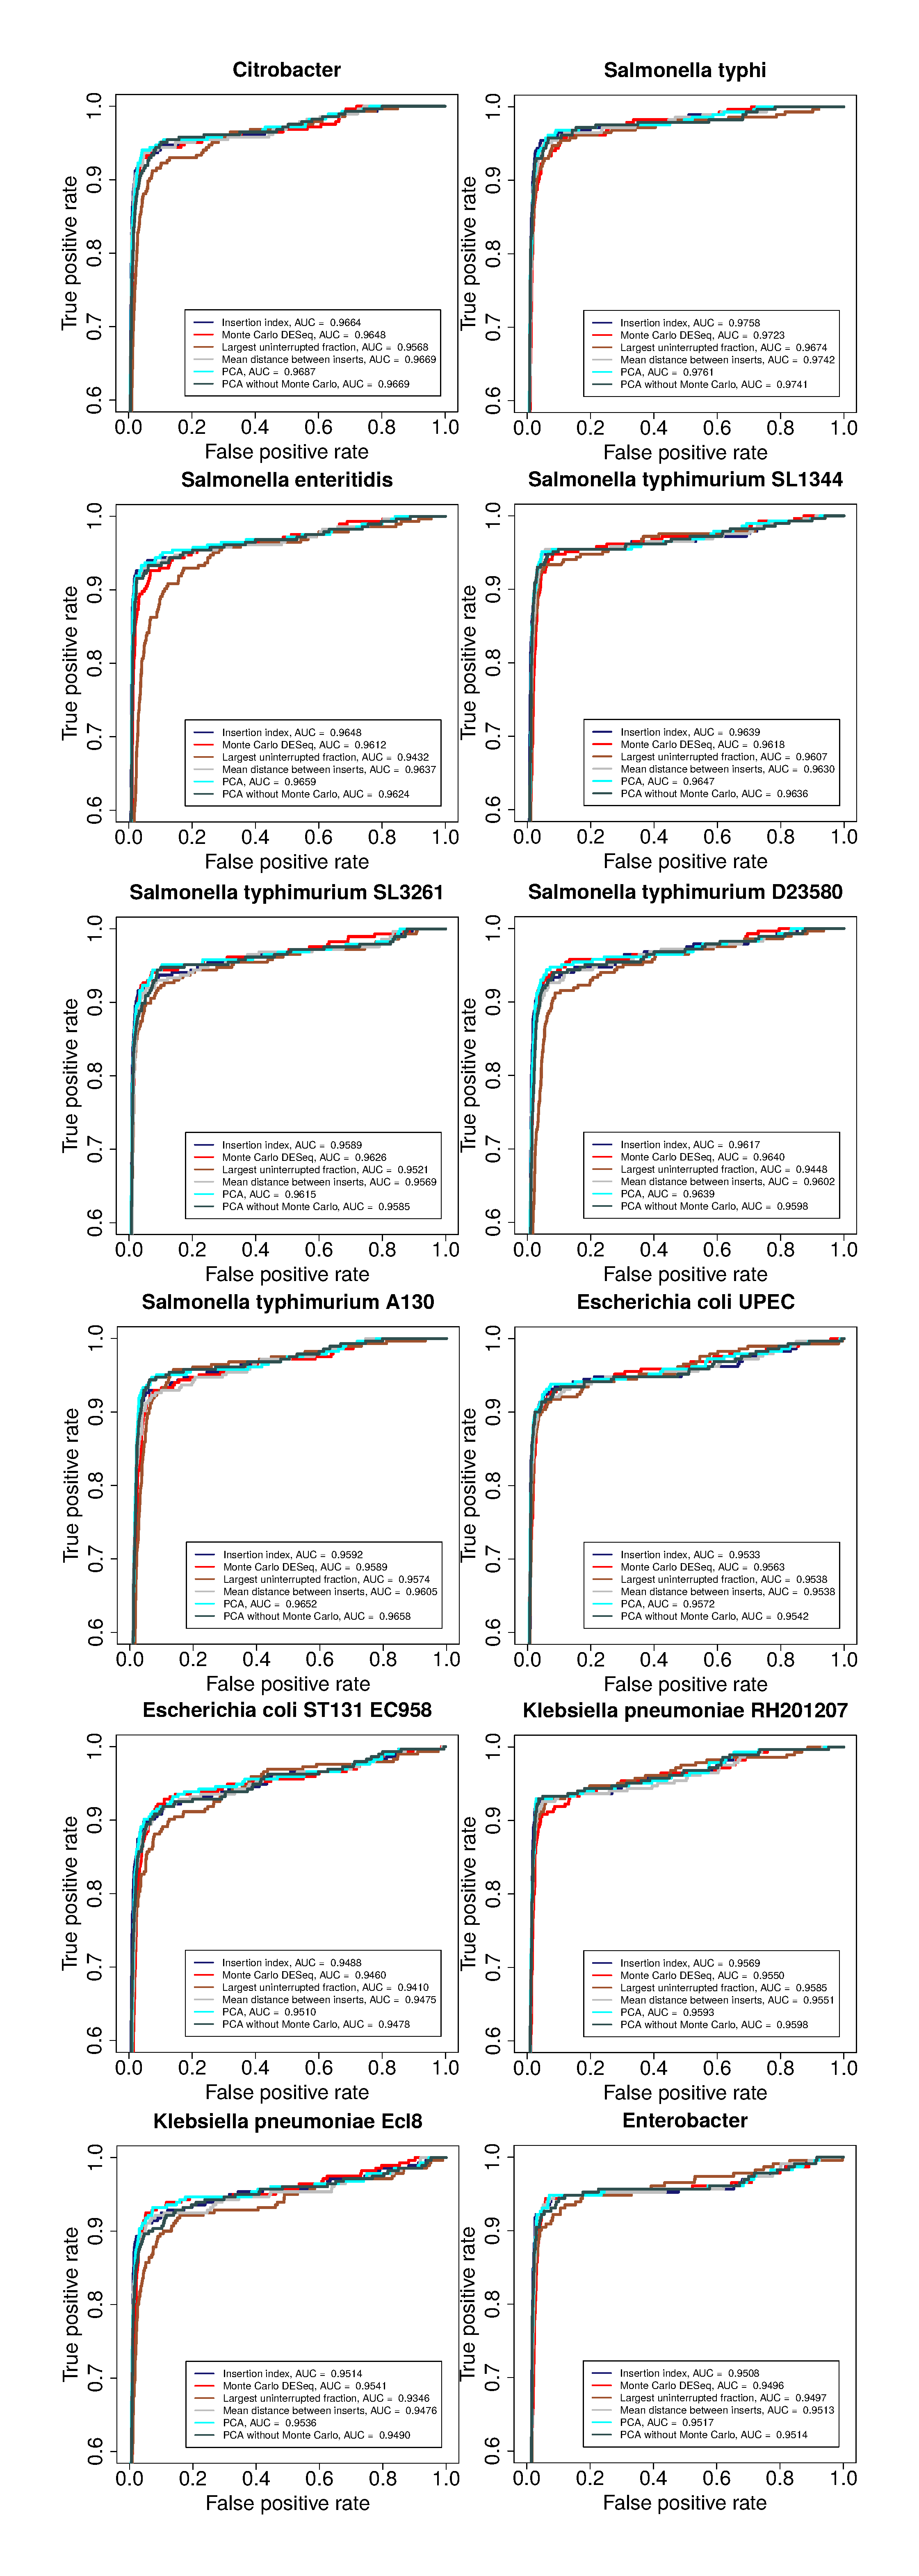
\includepdf[pages=1,fitpaper]{supplementary/supplementary.pdf}
\includepdf[pages=2,fitpaper]{supplementary/supplementary.pdf}
\includepdf[pages=3,fitpaper]{supplementary/supplementary.pdf}
\includepdf[pages=4,fitpaper]{supplementary/supplementary.pdf}
\includepdf[pages=5,fitpaper]{supplementary/supplementary.pdf}
\includepdf[pages=6,fitpaper]{supplementary/supplementary.pdf}
\includepdf[pages=7,fitpaper]{supplementary/supplementary.pdf}
\includepdf[pages=8,fitpaper]{supplementary/supplementary.pdf}
\includepdf[pages=9,fitpaper]{supplementary/supplementary.pdf}
\includepdf[pages=10,fitpaper]{supplementary/supplementary.pdf}
\includepdf[pages=11,fitpaper]{supplementary/supplementary.pdf}
\includepdf[pages=12,fitpaper]{supplementary/supplementary.pdf}
\includepdf[pages=13,fitpaper]{supplementary/supplementary.pdf}

\end{document}